\chapter{Microsecond molecular dynamics simulations for fragment pose prediction} \label{SEH-MD}

\small{Authors: Nathan M. Lim*, Linh P. Nguyen*, Gregory Warren, David L. Mobley}\\
\small{\textit{* denotes Co-First Authors}}

%%%%%%%%%%%%%%%%%%%%%%%%%%%%%%%%%%%%%%%%%%%%%%%%%%%%%%%%%%%%%%%%%%%%%
%% The abstract environment will automatically gobble the contents
%% if an abstract is not used by the target journal.
%%%%%%%%%%%%%%%%%%%%%%%%%%%%%%%%%%%%%%%%%%%%%%%%%%%%%%%%%%%%%%%%%%%%%
\section*{Abstract}
One of the major challenges medicinal chemists face in early drug discovery is the determination of ligand binding modes.
By understanding how a ligand orients itself within a binding site, chemists can gain insight on key interactions for binding and may begin to rationalize how to improve or design a potential lead compound. 
In this retrospective blinded study, we apply routine computational methods such as docking and molecular dynamics (MD) simulations to identify the binding modes on a set of fragment-like molecules bound to soluble epoxide hydrolase (sEH).
Here, we investigate each method's effectiveness in predicting the dominant binding mode and identifying any additional binding modes (if any), then validate our predictions to experimentally obtained X-ray crystal structures.
A set of 19 small molecules were docked into the apo protein crystal structure and then subsequently simulated for 1 microsecond each via MD.
To define ligand binding modes from our MD simulations, we construct Markov state models (MSMs) and analyze our results through a combination of Time-lagged Component Analysis (tICA) with Perron-clustering Cluster Analysis (PCCA).
We are particularly interested in determining whether exchanges between different stable binding modes can happen an adequate number of times at this timescale.
Given that these molecules are small and fragment-like, we expect switching of binding modes to occur relatively more quickly than typical drugs or biomolecules.
In this study, even with simulations at the microsecond timescale for small fragment-like molecules, we do not observe sufficient enough transitions to adequately sample and identify all crystallographic binding modes. 

\section{Introduction}
Early stage drug discovery commonly employs high-throughput screening (HTS), where millions of molecules (from small fragments to drug-like compounds) are screened against a target of interest to reveal potential hits.
However, HTS campaigns are expensive and often have low hit rates due to the vastness of chemical space and complexity of therapeutic targets \cite{erlanson_introduction_2012}.
Fragment-based drug discovery (FBDD) campaigns often begin their search through chemical libraries starting with smaller molecules (fragments) to cover a larger fraction of chemical space with the hope of yielding a higher probability of viable hits, even if initially less potent.
Hits obtained from FBDD are often weak binders but serve as a starting point for building lead compounds\cite{erlanson_tethering:_2004}.

Medicinal chemists typically use hits as a starting scaffold or connect fragments together in order to improve binding.
It is at this point in which determining the binding mode may be key for further improvement in the compounds' design \cite{gozalbes_contributions_2010}. 
Knowledge of how a fragment binds suggests key interactions to target for  improving binding and the consequences of scaffold modification.
It is also possible that a fragment may bind in several ways, whereby multiple binding modes contribute to the overall binding affinity \cite{stjernschantz_improved_2010}. 
Thus, in order to improve ligand binding affinity, a medicinal chemist must gain structural insight on the fragments binding mode or binding modes to have some guidance for further design and optimization.

Gaining structural insight to fragment binding modes by experimental methods often poses some challenges. 
Experimental methods for the determination of ligand binding modes include X-ray crystallography, nuclear magnetic resonance (NMR), and surface plasmon resonance.
However, these experimental methods can be costly, time-consuming, and difficult overall\cite{jhoti_fragment-based_2007, gozalbes_contributions_2010}.
Experimental methods such as X-ray crystallography often describe only the single (dominant) binding mode, if one is able to obtain crystals in high enough resolution.
The common problem in FBDD, with x-ray crystallography is that densities obtained in crystal structures can be ambiguous or in too low resolution to definitively resolve the binding mode of their compound.
Inherent to their size, small molecules and fragments often bind in multiple orientations which produce ambiguous densities in the crystal structure \cite{domagalski_quality_2014}.
This is where computational techniques and modelling may aid in the drug development process, by resolving ambiguities in crystal structures and predicted binding modes from computational techniques can help to make sense of partial occupancy data, helping to rescue structure-based design work for fragments.
When computational techniques become accurate enough, it could be employed even when structures aren't available\cite{erlanson_introduction_2012}.

Docking and molecular dynamics provide valuable tools to help determine fragment binding modes \cite{Rocklin2013BlindSite, durrant_computer-aided_2010, sliwoski_computational_2014}. 
Docking is a computationally inexpensive method that takes a static structure of a protein and places a given molecule in a variety of poses, generating a substantial number of candidate binding poses. 
This approach sacrifices accuracy but achieves high speeds by neglecting dynamics in the protein structure.
Although docking can be fast, there is difficulty in determining which of the generated candidate poses represent the relevant or true binding modes.
Dependent on the docking software used, each will score the placement of the ligand using a variety of metrics, usually based on fit within the binding site and scores which might provide rough estimates of protein-ligand interaction energies.
From docking scores, one may guess which molecules to carry forward to subsequent experiments, but docking scores are an unreliable metric for separating molecules that bind from those that do not bind \cite{lape_comparison_2010, plewczynski_can_2011, ramirez_is_2018, gohlke_knowledge-based_2000, warren_critical_2006}.
Docking has shown success in surveying the conformational space of the ligand, but has not proven completely accurate in producing experimentally discovered ligand binding modes \cite{guedes_receptorligand_2013, warren_critical_2006}.

Molecular dynamics (MD) is a computational method that solves Newton's equation of motions in discrete time steps to estimate the dynamics of the system, simulating in full atomistic detail the motions of a protein-ligand system over time \cite{hospital_molecular_2015, hollingsworth_molecular_2018}.
MD simulations allow protein dynamics to be studied in greater temporal and spatial resolution than experimental methods by simulating molecules in time steps compatible with the fastest motion in the system (i.e. bond vibration at 1-2 fs). 
Protein folding and other large conformational changes have timescales ranges from \(10^{-6}s\) (\(\mu\)s) to \(10^{0}\)s or slower \cite{han_protein_2014}. 
Atomistic MD simulations can routinely simulate timescales ranging from \(10^{-15}s\) (fs) to \(10^{-6}s\) (\(\mu\)s). 

Due to computational cost and lack of adequate conformational sampling, MD simulations are limited to shorter timescales than biologically relevant functions because a great amount of time steps are required to visualize these slow-order processes \cite{salmaso_bridging_2018}. 
In the case of FBDD, MD can capture the transition between ligand binding modes to reveal important stabilizing protein-ligand interactions on expected timescales ranging from nanoseconds to milliseconds.
In some cases, ligand binding mode transitions may even require conformational changes in the protein, where these timescales can go beyond milliseconds, however these longer timescales require a significant amount of computational resources  \cite{schlick_biomolecular_1997,macek_backbone_2007}.
This `timescale gap' between computational methods and biologically relevant timescales has been mediated by recent advancements towards increased sampling of the conformational space and Markov State Model (MSM) construction.
Here, we will evaluate whether sufficient sampling can even occur at the microsecond timescale using MD simulations and MSM construction.
Particularly, we are interested in determining if we can sufficiently sample enough binding mode transitions for our fragment set to obtain the correct populations and identify the dominant binding mode and/or additional binding modes.

\subsection{Fragment binding mode predictions to SEH} 
Soluble epoxide hydrolase (SEH) is a protein which is responsible for binding to specific epoxides, converting them to diols, and is found in nearly all tissues (but are highly concentrated in the liver).
The primary function of SEH is in detoxification, catabolism, and regulation of signaling molecules.
SEH catalyzes the breakdown of epoxyeicosatrienoic acids (EETs), acids with cardiovascular effects such as vasodilation and anti-inflammatory actions. 
Inhibition of SEH will slow the degradation of EETs, which can enhance neuroprotection, cardioprotection, and anti-inflammatory effects. 
In vitro studies with murine models have shown SEH inhibition significantly lowers blood pressure, supporting the hypothesized role of SEH in blood pressure regulation. 
The development of SEH inhibitors have therapeutic potential in cardiovascular diseases, inflammatory diseases, and neurological diseases. \cite{morisseau_impact_2013,morisseau_epoxide_2005,kodani_2014_2015}

In this retrospective study, we apply docking and MD techniques on a set of small fragment-like ligands in soluble epoxide hydrolase (SEH) in order to predict fragment binding modes.
We will determine whether docking and MD simulations can successfully identify the binding mode(s).
Binding modes are defined for the remainder of this paper as experimentally or simulation-determined metastable bound states.
Ligand poses are defined as the positions outputted from docking.
Prediction of ligand binding modes using a docking-MD combined approach has seen success in discriminating the experimental binding mode from challenging decoy poses, when compared to docking techniques alone \cite{liu_exploring_2017,clark_prediction_2016} and long MD simulations (e.g. 1 microsecond) have been used to visualize ligand entry and exit into the binding site \cite{decherchi_ligand_2015}.
Thus, we will evaluate whether 1 microsecond MD simulations provide any additional value after docking in uncovering additional ligand binding modes in this system.

The main objective of this study is to assess the performance of computational techniques such as docking and a combined docking and MD approach in identifying the relevant and dominant ligand binding modes (verified with experimental structures).
We aim to provide some insight to determine how effective computational methods can be in identifying the crystallographic binding mode, finding additional binding modes, or resolve ambiguities in experimental structures.

\section{Methods}

\subsection{Preparation}

\begin{figure}
    \centering
    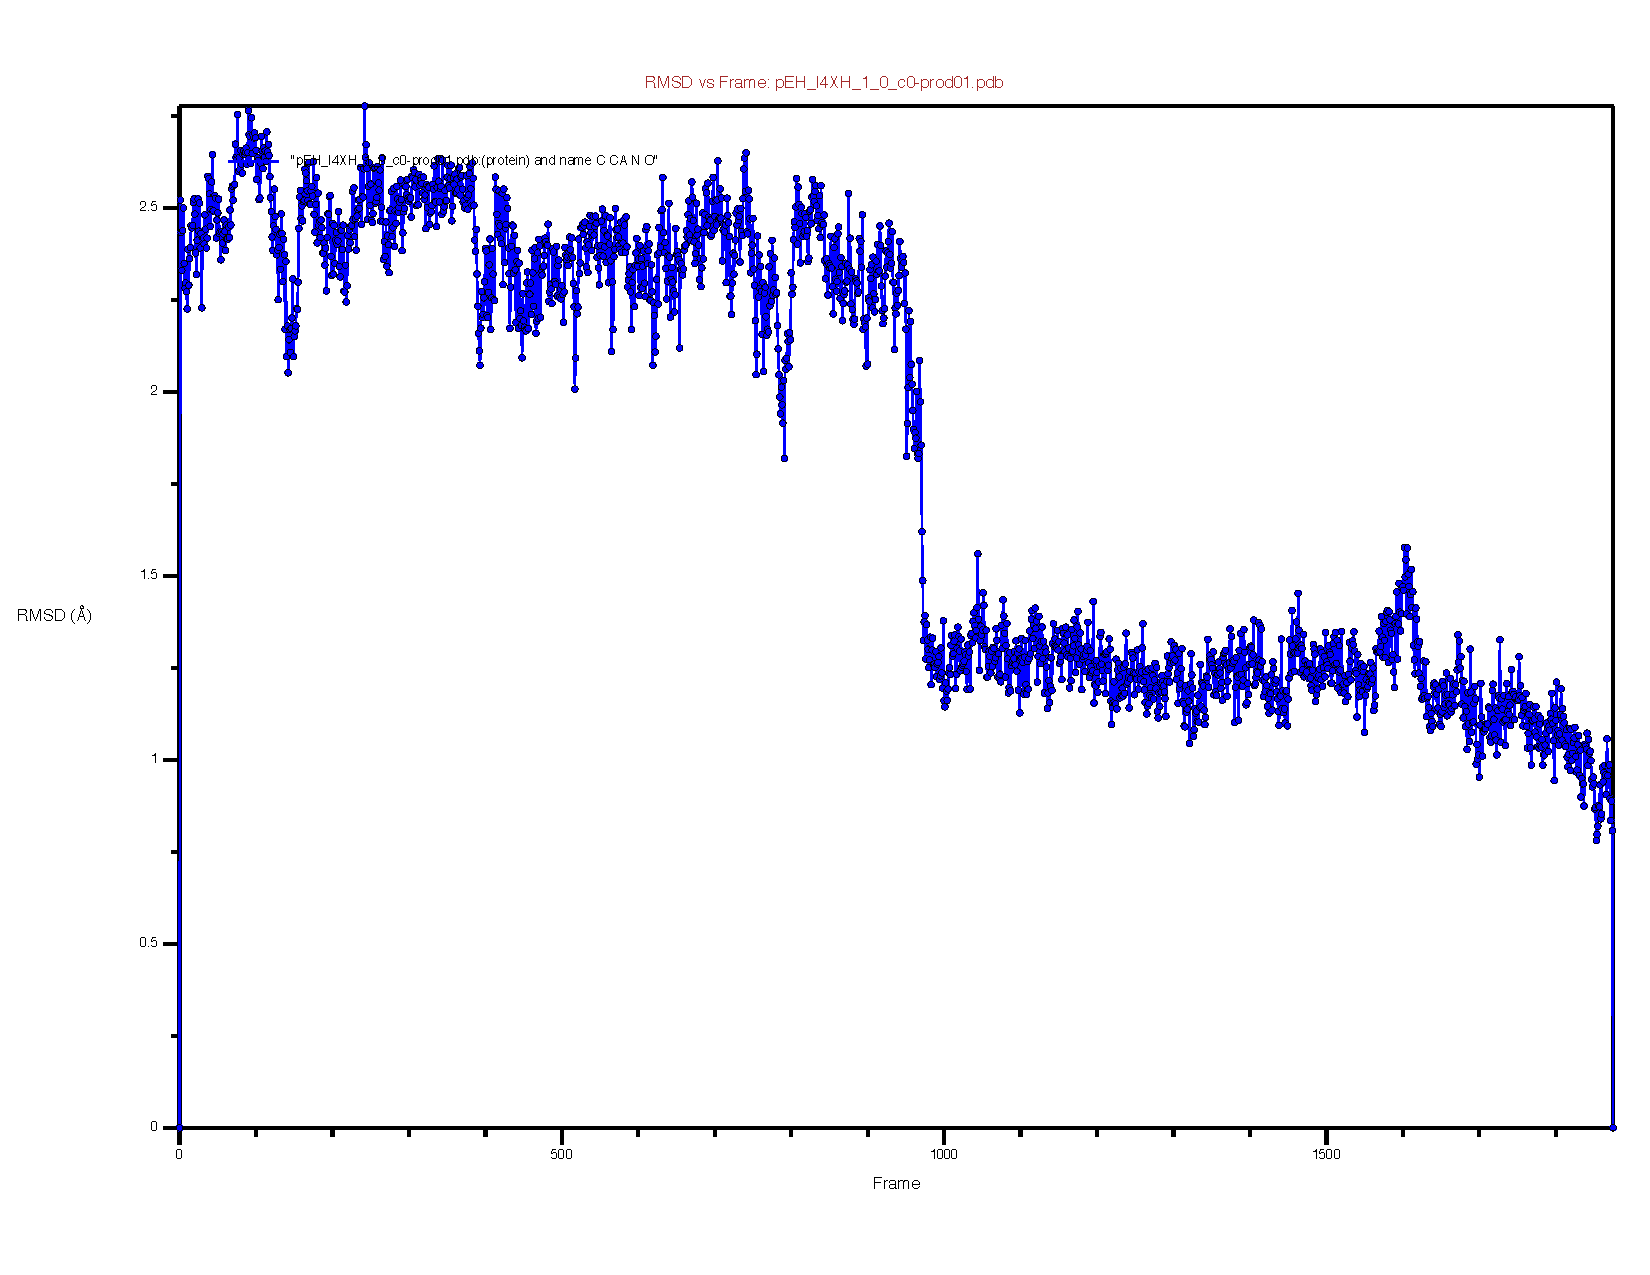
\includegraphics[width=\linewidth]{chapter5/Figures/backbonermsd.pdf}
    \caption[SEH Backbone RMSD]{RMSD of the SEH backbone, relative to the starting positions, after deleting the N terminal domain over the course of an 80ns MD simulation, averaging at 1.8{\AA}}
    \label{fig:backbonermsd}
\end{figure}
Information given to us by our OpenEye scientific collaborators (Christopher Bayly and Gregory Warren) consisted of the apo-protein SEH structure, the binding site in which to dock, the set of ligands to dock (given as SMILES strings), and the protein-ligand crystal structures after refinement by Warren.
All docking and MD simulations of the ligands were conducted without seeing the protein-ligand crystallographic structures.
The provided SEH structure contained missing residues and was not suitable input for MD simulations.
Instead, we used the apo structure of SEH taken from the Protein Data Bank (PDBID: 5AHX) and filled missing residues using PDBFixer \cite{noauthor_pdbfixer_2019}.

The apo SEH structure was uploaded to PDB2PQR \cite{} to strip waters from the system and assign protonation states at pH 8.5, as recommended by our collaborators, with AMBER parameters using PROPKA3.0\cite{jurrus_improvements_2018,sondergaard_improved_2011,noauthor_propka3:_nodate}. 
Parmed (v3.0.1) was used to convert the PQR file back to a PDB file by loading the structure then saving as a PDB \cite{swails_parameter/topology_2019}.
This corrected apo SEH structure was then aligned to the given SEH structure from OpenEye scientific to utilize the same defined binding site for docking.

The full SEH protein features two domains connected by a natural flexible linker, where the SEH binding site given to us was located in the C-terminal domain.
To reduce computational cost, the opposing domain which did not contain the pre-defined binding site was deleted from our simulated protein structure.
Specifically, resides 225 to 546 from the N-terminus of the protein system were deleted and the structural integrity of the protein was evaluated by analyzing the RMSD of the protein backbone.
The RMSD of the protein backbone averaged at 1.8 {\AA} over the course of a 80 ns MD simulation, indicating that deletion of the N-terminal domain did not affect the integrity of the C-terminal domain \ref{fig:backbonermsd}.
A similar trend in RMSD is observed when the N-terminal domain is retained.

\subsection{Docking}

A set of 47 ligands was obtained from collaborators at OpenEye Scientific which we separated into groups based on similarities in complexity. 
Using OpenEye packages to determine various molecular properties, the molecules were divided into 4 groups based on the number of rotatable bonds and their shape volume.
In this study, we examined the group with few rotatable bonds and small molecular volumes, which consists of 19 molecules.
Rotatable bonds for our data set range from 0 to 3 bonds and the volume of each molecule ranges approximately from 133\(\AA ^3\) to 172\(\AA ^3\).
We examined the group of small-fragment like molecules as we expected to observe more binding mode transitions within the microsecond timescale.
The remainder of the molecules will be reserved for subsequent studies.

\begin{figure}
    \centering
    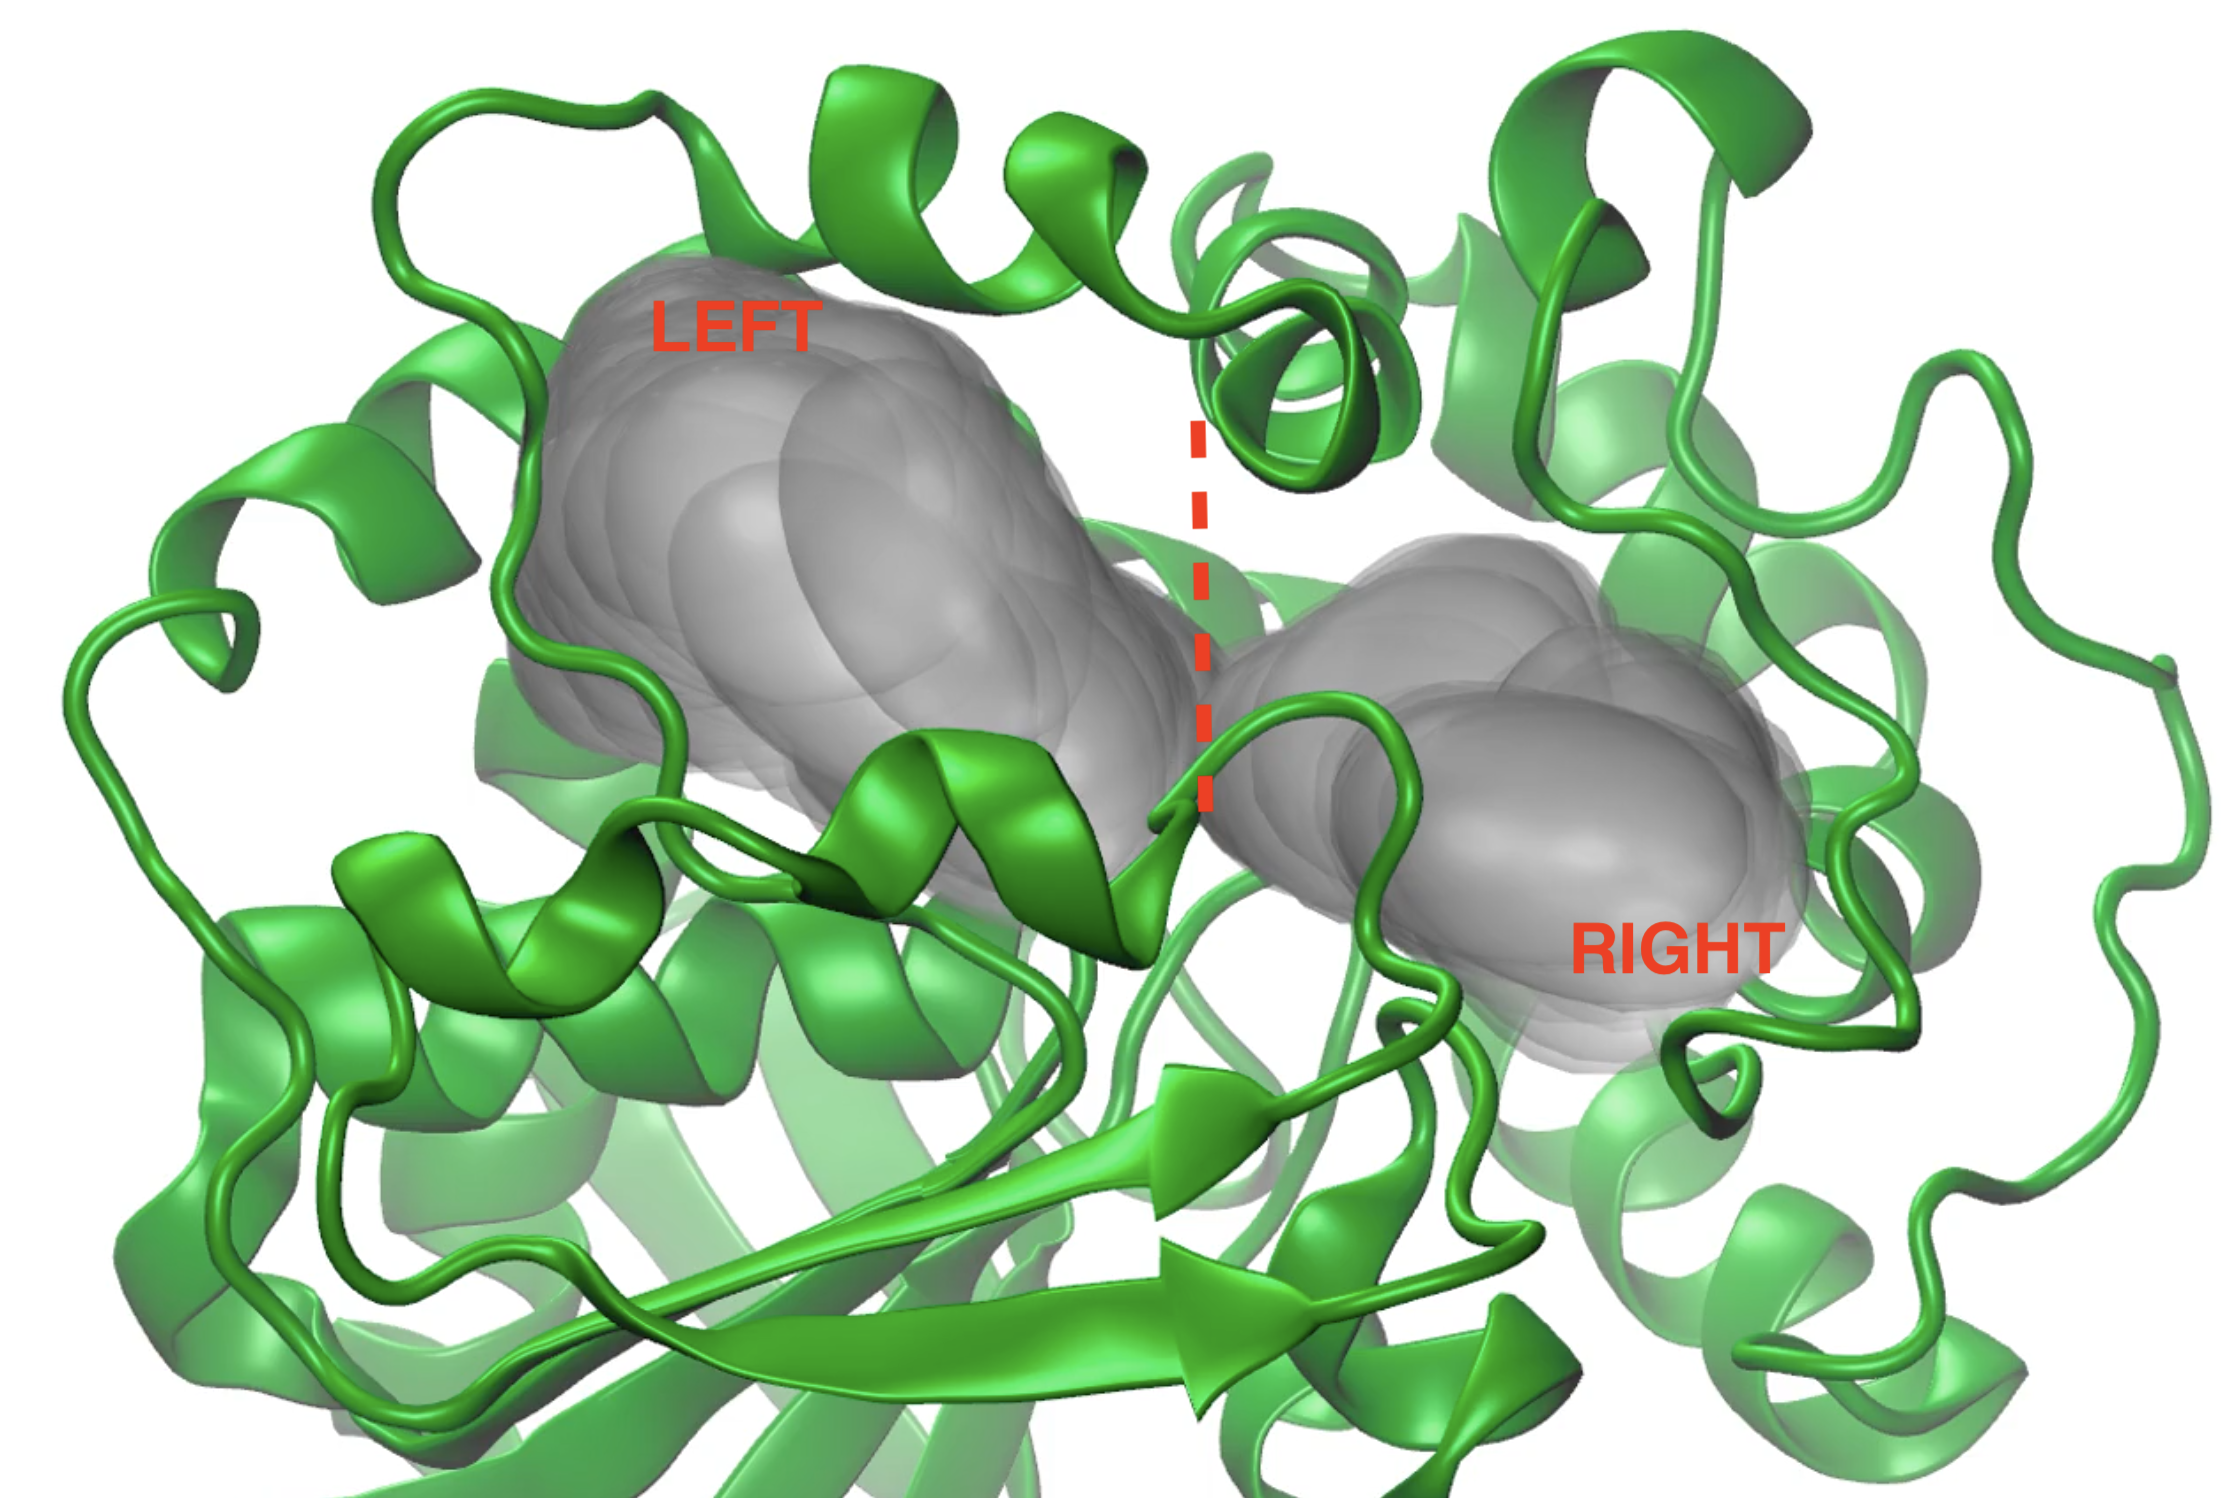
\includegraphics[width=\linewidth]{chapter5/Figures/seh-binding-site.png}
    \caption[SEH Binding Site]{Soluble Epoxide hydrolase binding site divided by the center cleft, defining two sub cavities denoted as left and right. As we rarely observed transitions between the two sub-caivities, we conduct our analysis of binding modes within each sub-cavity, shown here.}
    \label{fig:sEH-ribbon}
\end{figure}

\begin{figure}
    \centering
    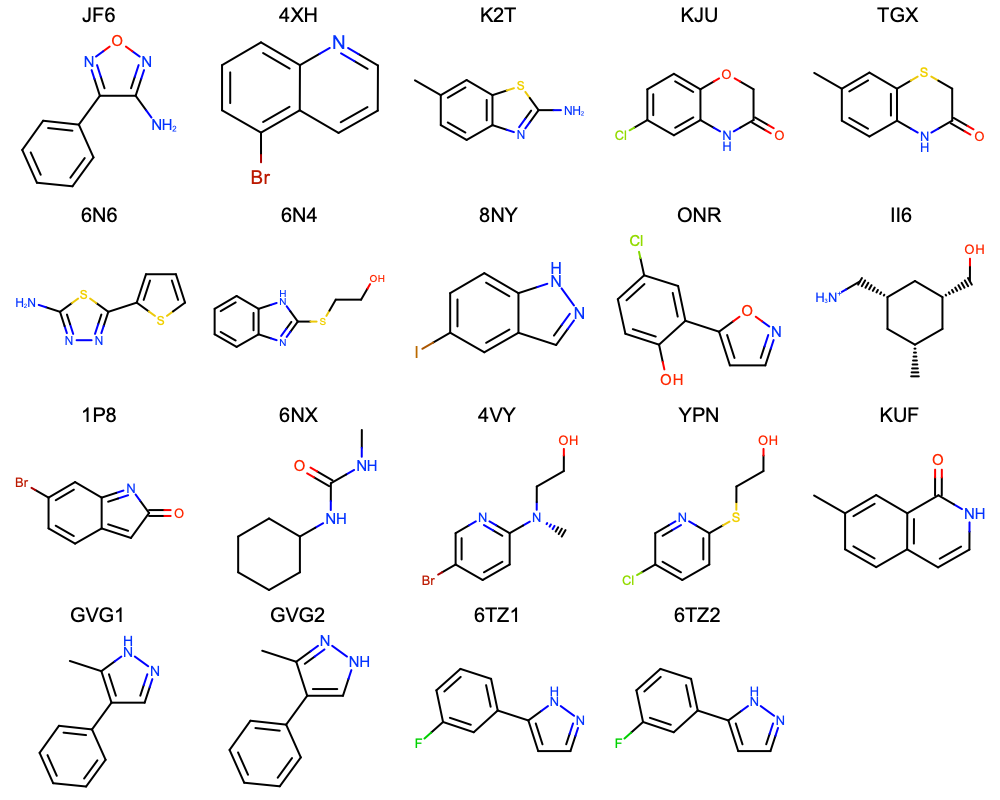
\includegraphics{chapter5/Figures/2d-molecules.png}
    \caption[SEH 2D Ligand Representation]{2D representations of the ligands used in this study. Each molecule is identified by a 3 character code, where alternate protonation states of select ligands are denoted with a 4 character code (i.g. GVG1/2, and 6TZ1/2). These codes are given to us by Warren.}
    \label{fig:2D-molecules}
\end{figure}

The 19 molecules (Fig. \ref{fig:2D-molecules}) were docked into the binding site, as defined by Warren, using the apo protein structure that we prepared for MD simulations.
In Figure \ref{fig:sEH-ribbon}, we divide the SEH binding site into two general regions (left and right) which are separated by two loops which form a cleft in the center \ref{fig:sEH-ribbon}.
At least one study on SEH has suggested that the left region of the binding site serves as a point of entry/exit to the catalytic domain on the right end of the binding side\cite{lotz_unbiased_2018}.

Using Openmoltools (0.8.3)\cite{eastman_openmm_2017} and OpenEye toolkits, each ligand's SMILES string was used to generate a 3D structure and assigned charges through the AM1BCCSym charging scheme via QUACPAC 2017.10.1 \cite{jakalian_fast_2002}. 
Then, we used OpenEye's OMEGA (20180212) to generate up to 1000 conformers for each ligand to be docked and scored\cite{hawkins_conformer_2010}.
The ligands (with their multiple conformers) were docked--into the docking region defined by Warren--using FRED through OEDock version 3.2.0.2. and then scored by the Chemgauss4 scoring function\cite{mcgann_fred_2011}.


From docking, 50 potential poses were generated and subsequently, up to 2-3 unique binding modes were hand-picked by visual inspection and used for the following for MD simulations.
The unique poses were selected to give us a variety of starting configurations for our MD simulations, and selecting docked poses that were in the different sub-cavities of the protein ensured reasonable coverage of all possible binding modes.
With enough simulation time, we expect the fragments to be able to transition between the sub-cavities and eventually find the correct binding mode.

\begin{figure}
    \centering
    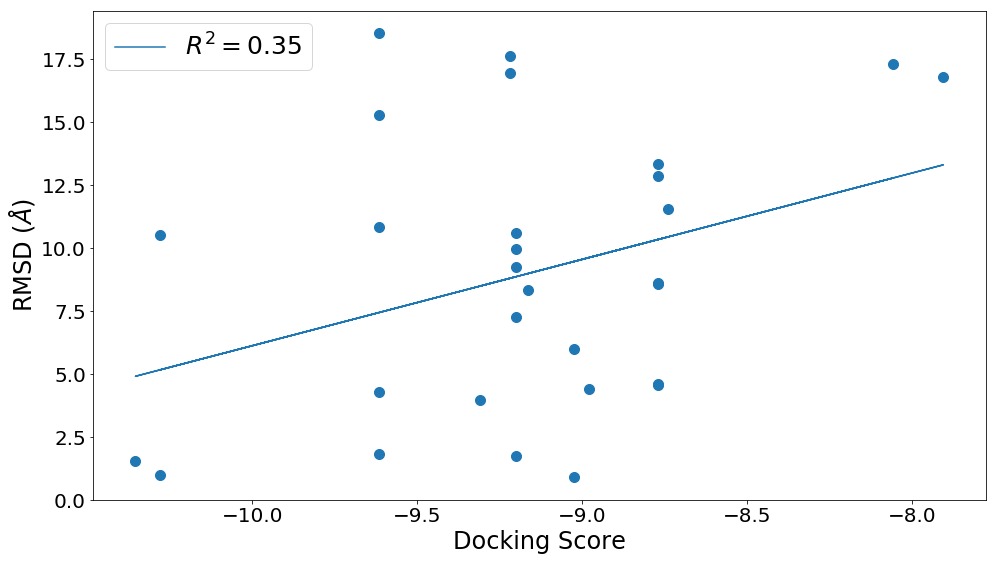
\includegraphics[width=\linewidth]{chapter5/Figures/topscore-rmsd.png}
    \caption[RMSD of Top Scoring Docked Poses]{Relationship between the top scoring pose from docking and RMSD to the crystallographic binding mode. Scores from docking do not correlate with the closeness to the crystallographic pose.}
    \label{fig:topscore_correlation}
\end{figure}

The choice to manually select docked poses for increasing the variety of starting MD configurations over selecting poses with the highest docking score is based on the assumption that the docking score is a poor metric for identifying the actual binding mode \cite{warren_critical_2006}.
Figure \ref{fig:topscore_correlation}, illustrates the calculated RMSD of the top scoring poses in this study, does not correlate with closeness to the crystallographic binding mode.
This finding validates our choice to utilize manual selection of the docked poses for starting our MD simulations.

\subsection{Molecular Dynamics}
The system, compromising of only the C-terminal domain, was parameterized using amber99sbildn force field for the protein \cite{wang2004development}, the TIP3P water model \cite{jorgensen1983comparison} for the solvent, and GAFF2 force field for the ligands \cite{lindorff-larsen_improved_2010}.
The following stages were carried out using OpenMM (version 7.1.1) \cite{eastman_openmm_2017,eastman_openmm_2013}.
A maximum of 30,000 minimization steps was applied and the protein-ligand system was equilibrated for 10ps at 1 atm, 300K, and a pH of 8.5 in three stages where the restraint force used to keep the ligand and protein in their starting positions is decreased with each progressing stage. 
The restraint force constant for each progressive stage was $2.0 \frac{kcal}{mol \cdot \mbox{\AA} ^{2}}$, $0.5 \frac{kcal}{mol \cdot \mbox{\AA} ^{2}}$, and $0.1 \frac{kcal}{mol \cdot \mbox{\AA} ^{2}}$, respectively. 
Unrestrained molecular dynamics simulations of the protein-ligand system were then carried out for 1 microsecond for each of the chosen docked poses.

\subsection{Determining Binding Modes by TICA and PCCA}
From our 1 microsecond MD simulations, we rarely observed transitions between the two sub-cavities.
Thus, we divided the analysis of our simulations, separately analyzing cases where the starting pose was in the left sub-cavity and those where the poses were started in the right sub-cavity.
By separating analysis between each respective side of the binding site, we are able to better distinguish between different binding modes sampled during the course of the simulation. 
This allows us to better understand the transitions among these binding modes rather than the timescale to transition between the two sub-regions in the binding site.
For the rare cases in which we observed transitions between the sub-cavities, the simulation data was treated collectively.
Analysis was conducted on the entirety of the 1 microsecond simulation, with trajectory frames stored for analysis every 40ps.

\begin{figure}
    \centering
    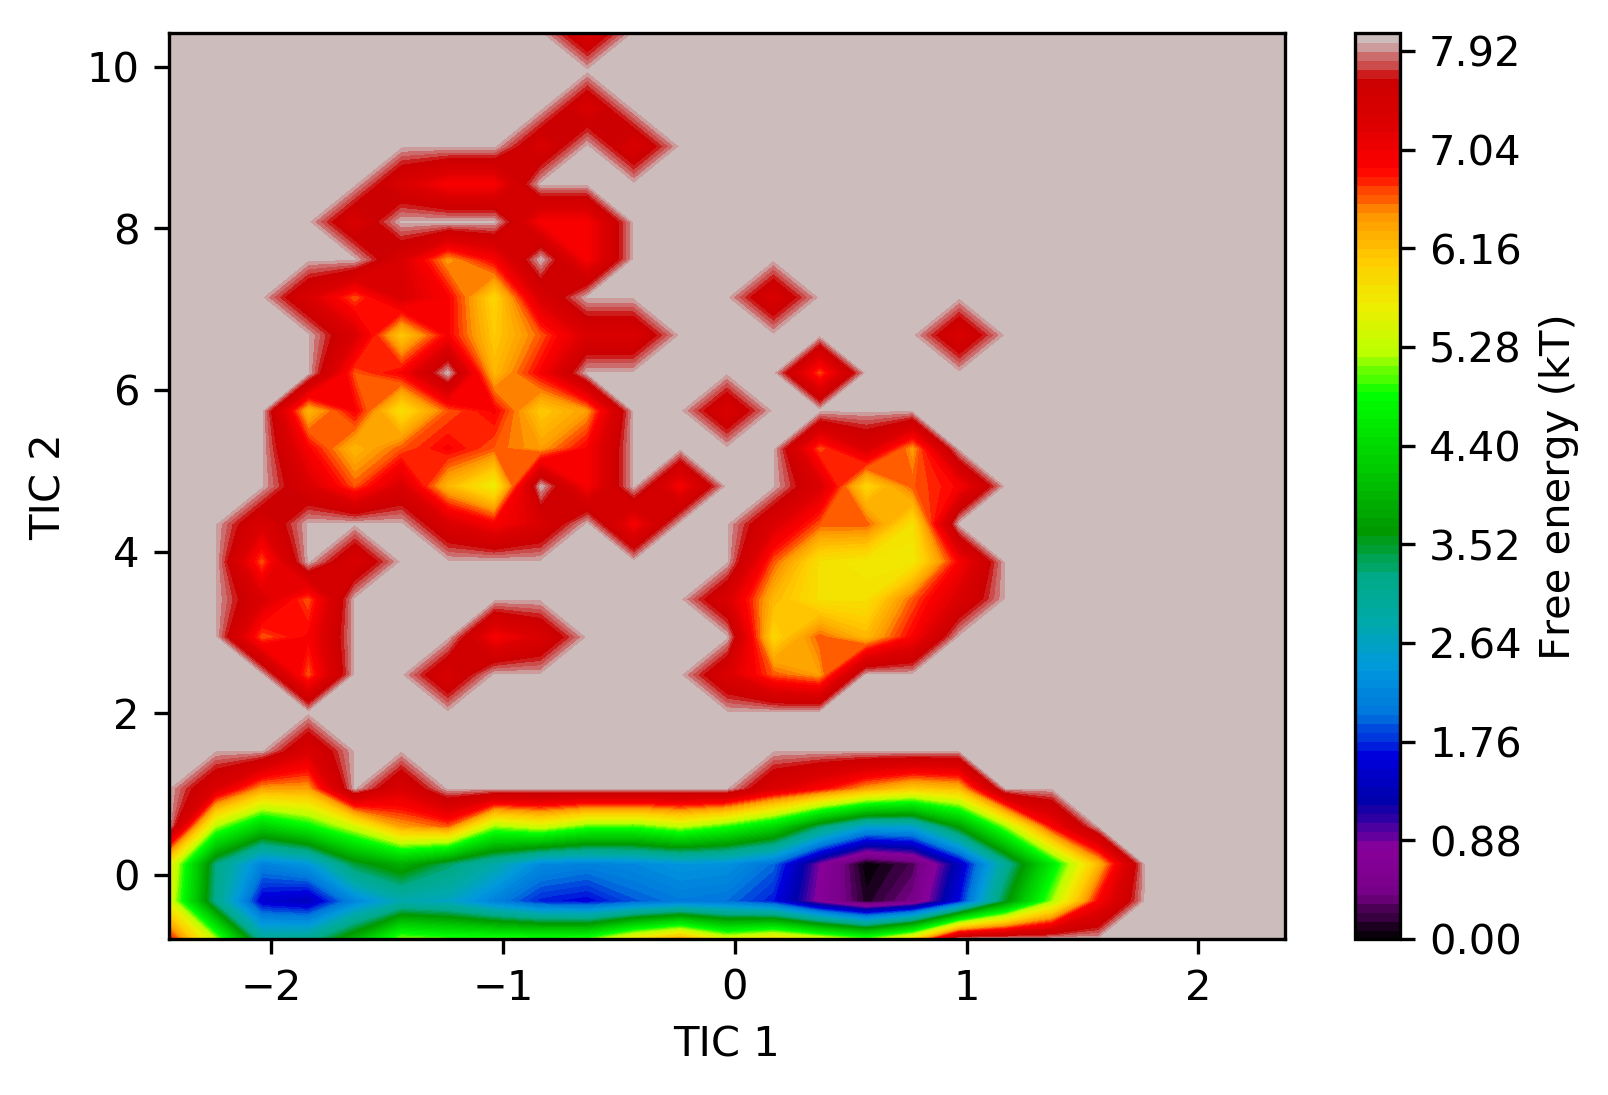
\includegraphics{chapter5/II6/II6_1-full-tiCA.png}
    \caption[TICA Analysis of Ligand II6]{TICA analysis of the conformational dynamics of ligand II6 during a 1 microsecond MD simulation yields three possible metastable binding modes as recognized by the (blue, violet, or black) metastable free energy basins.}
    \label{fig:II6_1_tica-kmeans}
\end{figure}

We use PyEMMA (v2.5.2) to analyze the ligand binding modes sampled during our 1 microsecond MD simulations and used the results to construct Markov State Models (MSM)\cite{scherer_pyemma_2015}. 
Here, we chose the distance from the closest heavy ligand atom to key residues as our feature set and apply time-lagged independent component analysis (tICA) \cite{perez-hernandez_identification_2013} to determine the slowest order parameters. 
Previous studies on the SEH system suggested key residue-ligand interactions were among residues ASP110, TYR158, MET194, TYR241, and VAL273 \cite{lotz_unbiased_2018}. 
After applying a tICA transformation on the distances from the closest heavy ligand atom to key residues, we then used the first two TICA components and generate discrete microstates by k-means clustering (Figure \ref{fig:II6_1_tica-kmeans}).

\begin{figure}
    \centering
    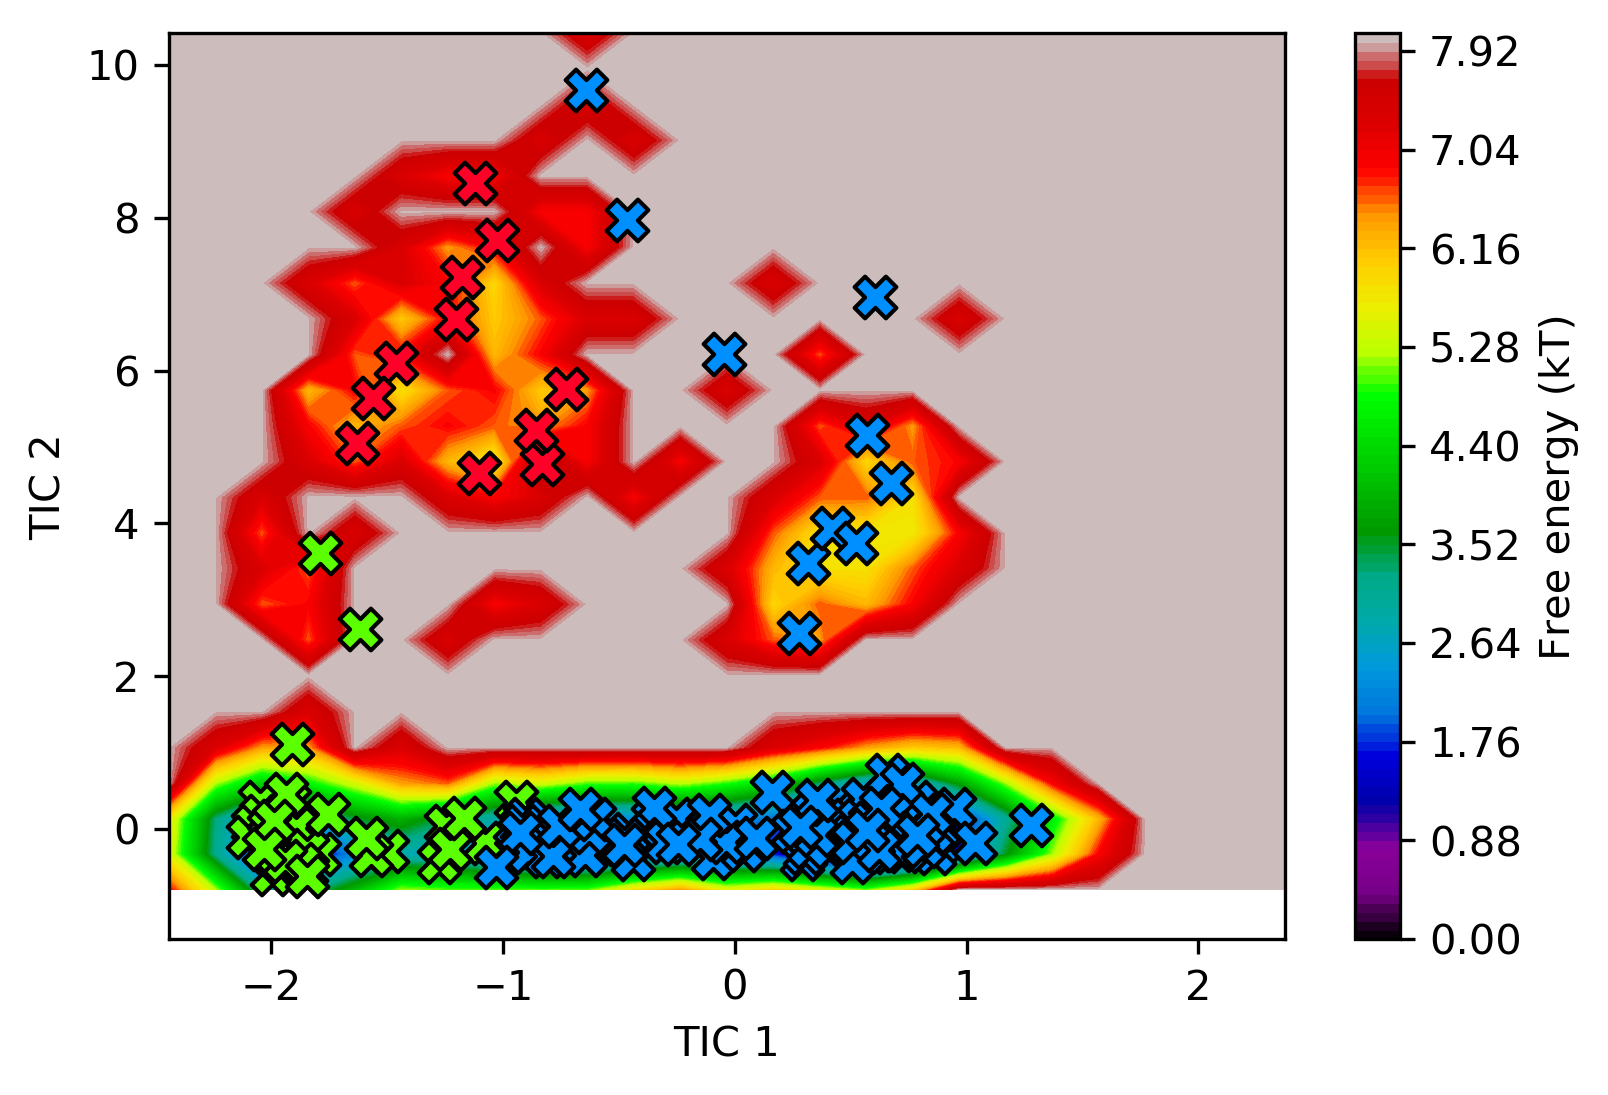
\includegraphics{chapter5/II6/II6_1-full-tiCA-PCCA.png}
    \caption[PCCA Analysis of Ligand II6]{Ligand II6 TICA coordinates plot with marked discrete microstates colored to indicate different clusters which define our metastable macrostates or stable ligand binding modes. Adjacent macrostates suggest possible transitions between binding modes.}
    \label{fig:II6_1-TICA-PCCA}
\end{figure}

In tICA space, we plot N discrete microstates (representing individual simulation frames), where N is the square root of the total number of simulation frames (i.e. 5000 simulation frames). 
Following this, we build up our macrostates by assigning each discrete microstate to a macrostate using perron-cluster cluster analysis (PCCA) \cite{roblitz_fuzzy_2013,deuflhard_robust_2005} (Figure \ref{fig:II6_1-TICA-PCCA}).
For each macrostate, we store 100 frames to represent our metastable binding modes sampled from MD.


\begin{figure}
    \centering
    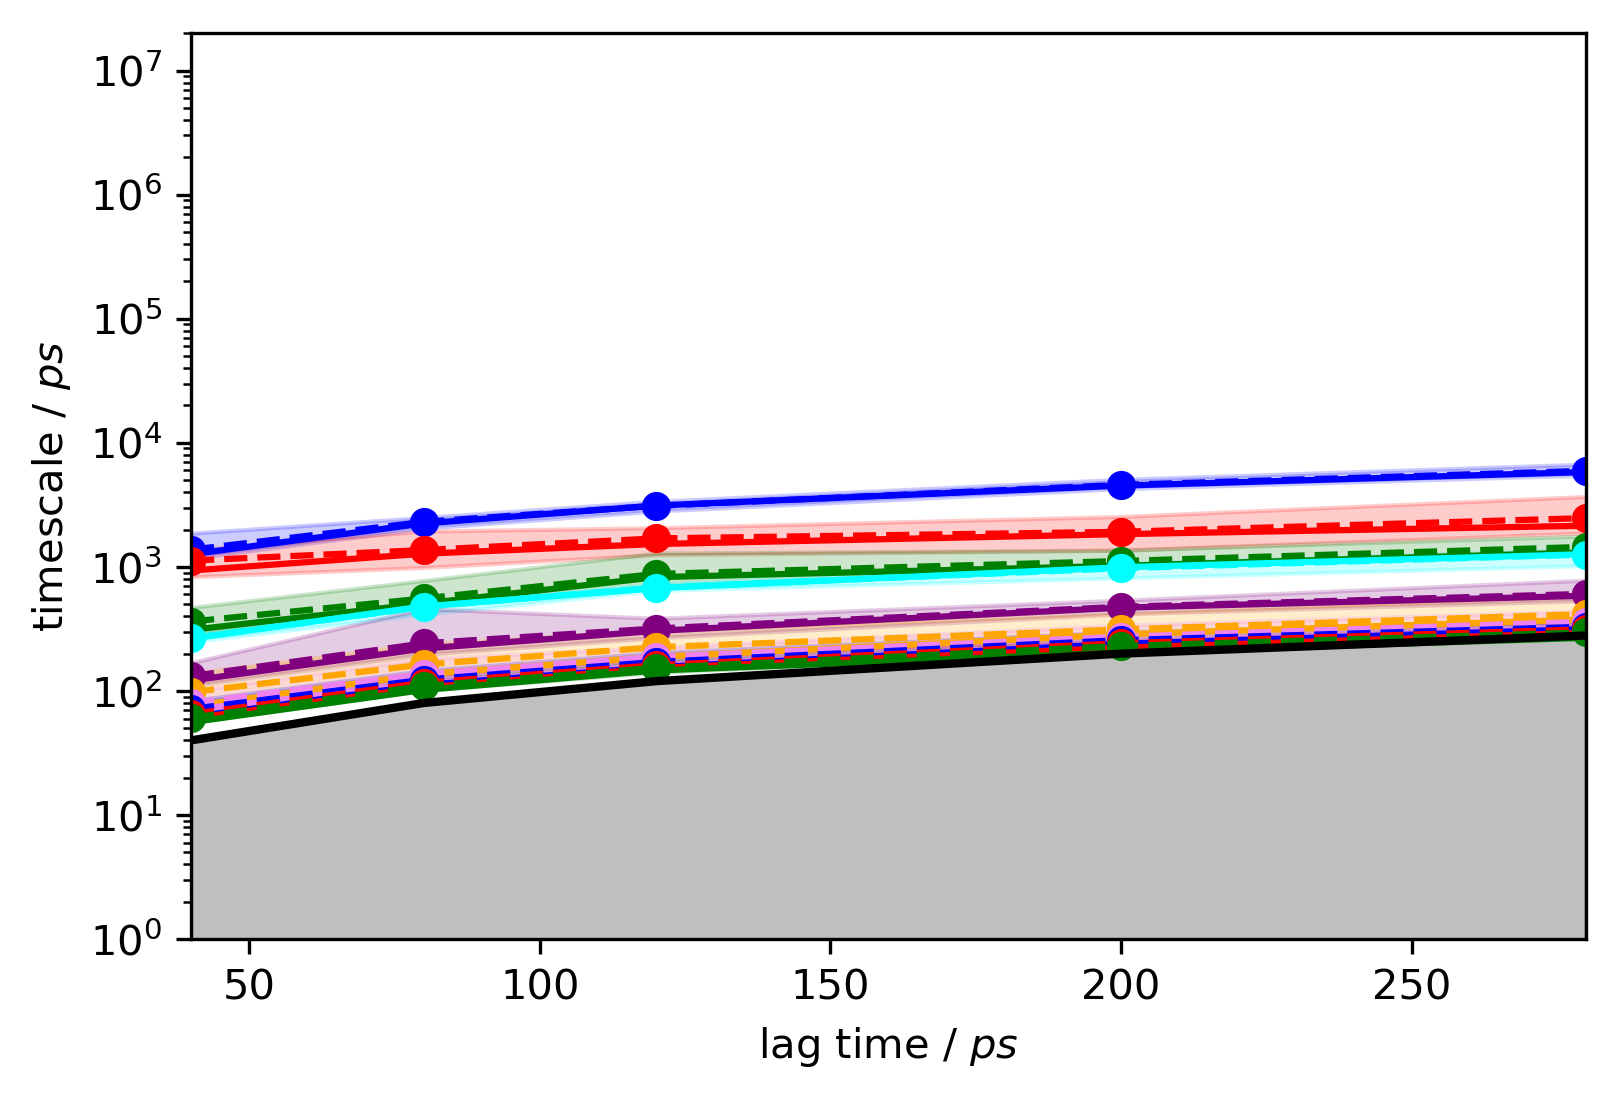
\includegraphics{chapter5/II6/II6_1-full-implied-timescale.png}
    \caption[SEH Implied Timescales]{Relaxation timescales of ligand II6 implied by a Markov model transition matrix estimated at various lag times up to 300ps. Implied timescales should be independent of the lag time and appear to converge at 100ps. With increasing lag time, implied timescales become more constant. The black line with gray area defines the limit of the timescale at which the model can be resolved, where any processes within this area are generally not resolved. With increasing lag time, more process are not resolved. All the processes for II6 are well resolved. Solid lines correspond to the maximum likelihood MSMs. Shaded areas depict confidence intervals containing 95 percent of the samples generated by Bayesian MSM. The confidence intervals remain constant with increasing lag time for II6. Dashed lines correspond to samples means. }
    \label{fig:II6-implied}
\end{figure}

Choosing an appropriate lag time is crucial in properly analyzing the MD trajectories, where a long lag time may gloss over significant ligand movement and a short lag time may unnecessarily be computationally expensive.
The implied timescales provided insight on the timescales to transition into different states.
Plotting the implied timescales against lag time helps select an MSM lag time that will be long enough to indicate Markovian dynamics and short enough to resolve the processes \cite{wehmeyer_introduction_2018}.
A lag time of 300ps was selected as the implied timescale appeared to become independent of lag time (Figure \ref{fig:II6-implied}). 

\begin{figure}
    \centering
    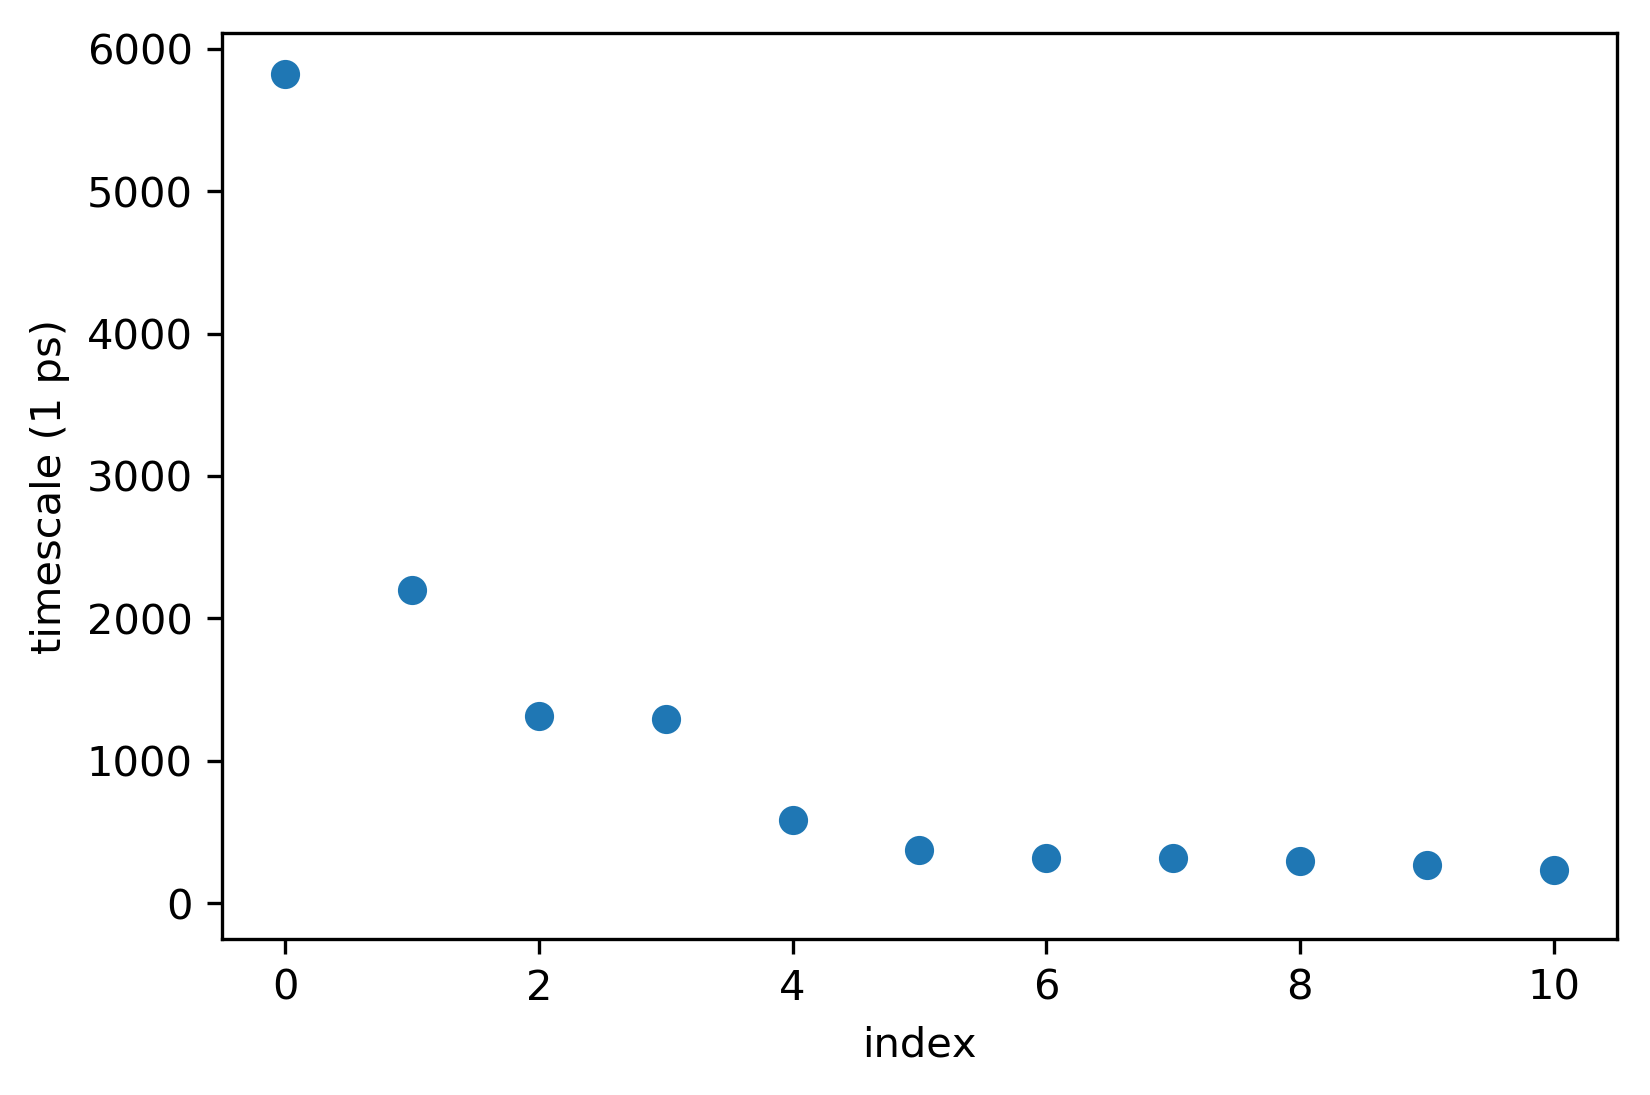
\includegraphics{chapter5/II6/II6_1-full-spectra.png}
    \caption[Spectral Analysis of Ligand II6]{Ligand II6 number of clusters against their respective MSM timescales. With increased clusters, the duration of the timescale each cluster represents decreases. Using the elbow method, we select the number of clusters that will best separate the discrete microstates into macrostates. A suitable number of clusters appears to be 3 clusters. }
    \label{fig:II6_1-spectral}
\end{figure}

The number of metastable states was determined from spectral analysis by plotting the number of clusters vs. their respective timescales, then selecting the number of appropriate clusters based on the elbow method (Figure \ref{fig:II6_1-spectral}).

To illustrate the change in binding modes over time, we plot the ligand RMSD from the starting frame and color each time point by the minimizing the RMSD from our 100 frames representing each macrostate or our metastable binding modes.
We then calculate the populations by computing the frequency or the amount of simulation time spent in each defined binding mode.
This effectively shows the occupancy of each binding mode during the 1 microsecond MD simulation and the RMSD of the ligand over time \ref{fig:II6_bmodes} from the initial docked pose.

\subsection{Comparison to the crystallographic pose}
We evaluated docking and MD for their effectiveness in determining ligand binding modes by calculating the RMSD to the crystallographic pose.
Given our (validated) assumption that docking scores does poorly in indicating closeness to the crystallographic binding mode (Fig. \ref{fig:topscore_correlation}), we have no way of knowing which single pose would minimize the RMSD.
The docked poses simulated in MD should not represent docking RMSD because the docked poses were selected based on increasing the variety of starting configurations for MD and are irrelevant to docking abilities in effectively predicting ligand binding modes.
Reporting the RMSD of the best single docked pose would bias the results in favor of docking and not accurately represent the process of using docking to determine ligand binding modes but would show a rare best case scenario of utilizing docking.
Thus, we report the average RMSD from docking to best represent selecting a pose at random from a pool of generated docked poses.
For docking, we computed the average RMSD (with confidence intervals at 95\%) by randomly drawing 50,000 docked poses (without replacement) from our initial 50 generated docked poses.

Similarly, for MD, we report the average RMSD (with confidence intervals at 95\%) by randomly drawing 10,000 frames from our 100 frames we saved as are representatives of each binding mode sampled from MD.
Average MD RMSD values were calculated to best represent the process of selecting a single frame at random from each macrostate, which represent the metastable binding modes sampled during our MD simulations.
Since we do not know which frame sampled during our MD simulation would minimize the RMSD to the crystallographic binding mode, we cannot report the minimum RMSD from our MD simulations.

In cases where the molecule had a single crystallographic binding mode, the most populated cluster was selected as the predicted pose from MD.
In cases where the molecule had two crystallographic binding mode, the top two populated clusters were selected to represent the predicted binding modes from MD.
In cases where the molecules had multiple crystallographic binding modes, we present the average RMSD of each macrostate that minimizes the computed RMSD to the crystallographic binding mode.
Given that we did not know ahead of the study whether any given molecule would exhibit more than two binding modes in crystallography, nor did we observe more than 3 binding mode transitions in our simulations, we believe our procedure for analysis represents a fair assessment for a blind prediction challenge.
Experimental MD ligand pose RMSD values within 2{\AA} of the crystallography binding mode were considered to have sufficiently predicted the binding mode \cite{warren_critical_2006} \cite{plewczynski_can_2011}. 

We remind the reader that we started simulations using poses from each sub-cavity in the SEH binding site and if the crystallographic pose was only found in one sub-cavity, we discarded the simulation data in the opposing sub-cavity--except if we saw transitions between sub-cavities in our simulations.
Given that we rarely observed transitions between sub-cavities in our 1 microsecond MD simulations, in some sense, our predictions put forth represent an `ideal' scenario, where one knows which sub-cavity that the molecule may bind in before running their simulations. 
In subsequent work we hope to explore methods to enhance the transition rate between sub-cavities.

\section{Results}
Given that we do not know ahead of time which docked pose or simulation frame would minimize the RMSD, we remind the reader that we report average RMSDs to replicate the scenario of randomly picking a docked pose or a single simulation frame from MD to compare against the crystal structure (See Methods:Comparison to the crystallographic pose).

\subsection{Single binding mode predictions}
\begin{figure}
    \centering
    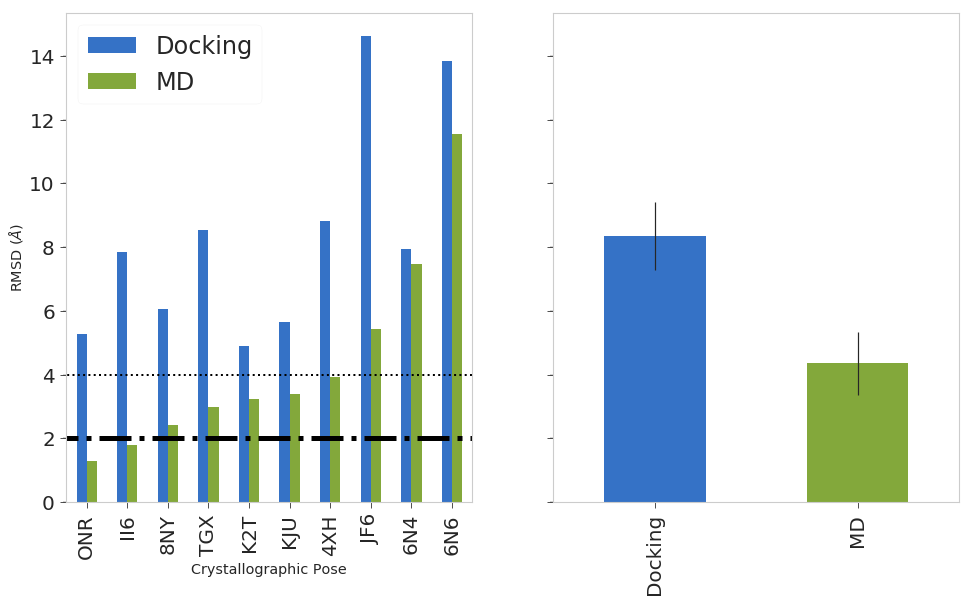
\includegraphics[width=\linewidth]{chapter5/Figures/cluster3_seh_singlebm.png}
    \caption[SEH MD Single Binding Mode Ligands]{RMSD between crystallographic ligand binding mode and predicted binding mode from docking (blue) and MD (green) for cases with a single crystallographic binding mode. Ligand RMSD values are sorted in ascending order according to MD RMSD. We judge success as predicting a binding mode to be less than or equal to 2 {\AA} (black dashed horizontal line). For ligands with single binding modes, MD simulations generally improve RMSD values from docking.}
    \label{fig:rmsd-singlebm}
\end{figure}

\begin{table}[]
\begin{tabular}{|l|l|l|l|l|}
\hline
\textbf{Ligand} & \textbf{Dock} & \textbf{DockErr} & \textbf{MD} & \textbf{MDErr} \\ \hline
\textbf{JF6}    & 14.6          & \textit{0.1}     & 5.4         & \textit{0.1}   \\ \hline
\textbf{4XH}    & 8.8           & \textit{0.1}     & 3.9         & \textit{0.0}   \\ \hline
\textbf{KJU}    & 5.7           & \textit{0.0}     & 3.4         & \textit{0.0}   \\ \hline
\textbf{TGX}    & 8.5           & \textit{0.1}     & 3.0         & \textit{0.0}   \\ \hline
\textbf{6N6}    & 13.8          & \textit{0.0}     & 11.5        & \textit{0.2}   \\ \hline
\textbf{6N4}    & 7.9           & \textit{0.0}     & 7.5         & \textit{0.1}   \\ \hline
\textbf{8NY}    & 6.1           & \textit{0.0}     & 2.4         & \textit{0.0}   \\ \hline
\textbf{ONR}    & 5.3           & \textit{0.0}     & 1.3         & \textit{0.0}   \\ \hline
\textbf{II6}    & 7.8           & \textit{0.1}     & 1.8         & \textit{0.0}   \\ \hline
\textbf{K2T}    & 4.9           & \textit{0.0}     & 3.2         & \textit{0.0}   \\ \hline
\end{tabular}
\caption{Average RMSDs and error {\AA} for molecules with a single binding mode.}
\label{table:singlebm}
\end{table}


Molecules JF6, 4XH, KJU, TGX, 6N6, 6N4,  8NY, ONR, II6, and K2T each had single crystallography binding mode.
Docking had an average RMSD ({\AA}) of 14.63, 8.82, 5.65, 8.52, 13.83, 7.95, 6.06, 5.27, 7.85, and 4.90 for the molecules respectively.
Our reported confidence intervals (at 95\%) for the average RMSDs for each molecule was under 0.05 {\AA}.
The average RMSD ({\AA}) from the most populated binding mode during MD was 5.43, 3.93, 12.09, 2.97, 11.54, 7.46, 2.43, 1.30, 1.79, 3.24, for the molecules respectively.
These values are noted in Table \ref{table:singlebm}.
None of the molecules with single binding modes yielded an average docking RMSD under the 2 {\AA} cutoff.
From MD, 2/10 molecules (ONR and II6) had an average RMSD under the 2 {\AA} cutoff for ligands.
The average docking RMSD for molecules with a single binding mode was $8.3 \pm 1.1 {\AA}$.
The average MD RMSD for molecules with a single binding mode was $4.3 \pm 1.0 {\AA}$.

\subsection{Dual binding mode predictions}
\begin{figure}
    \centering
    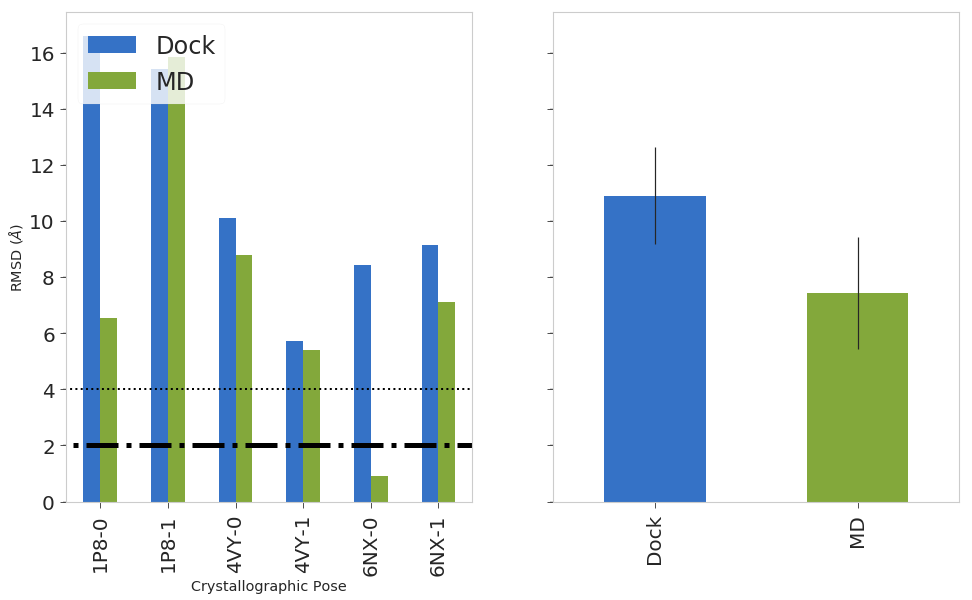
\includegraphics[width=\linewidth]{chapter5/Figures/cluster3_seh_dualbm.png}
    \caption[SEH MD Dual Binding Mode Ligands]{RMSD between crystallographic ligand binding modes and predicted binding modes from docking (blue) and MD (green) for cases with dual crystallographic binding modes. We judge success as predicting a binding mode to be less than or equal to 2 {\AA} (black dashed horizontal line). }
    \label{fig:rmsd-dualbm}
\end{figure}

\begin{table}[]
\begin{tabular}{|l|l|l|l|l|}
\hline
\textbf{Ligand} & \textbf{Dock} & \textbf{DockErr} & \textbf{MD} & \textbf{MDErr} \\ \hline
\textbf{1P8-0}  & 16.6          & \textit{0.0}     & 6.5         & \textit{0.0}   \\ \hline
\textbf{1P8-1}  & 15.4          & \textit{0.0}     & 15.8        & \textit{0.1}   \\ \hline
\textbf{4VY-0}  & 10.1          & \textit{0.0}     & 8.8         & \textit{0.0}   \\ \hline
\textbf{4VY-1}  & 5.7           & \textit{0.0}     & 5.4         & \textit{0.0}   \\ \hline
\textbf{6NX-0}  & 8.4           & \textit{0.0}     & 0.9         & \textit{0.0}   \\ \hline
\textbf{6NX-1}  & 9.1           & \textit{0.0}     & 7.1         & \textit{0.0}   \\ \hline
\end{tabular}
\caption{Average RMSDs and error {\AA} for molecules with two binding modes.}
\label{table:dualbm}
\end{table}


Molecules 6NX, 4VY, and 1P8 each had two crystallographic binding modes.
Average docking RMSD values against the two crystallographic binding modes for each molecule were 16.6 \& 15.4 (6NX), 10.1 & 5.7 (4VY), and 8.4 \& 9.1 (1P8).
The average RMSD from the top two most populated binding modes from MD were 6.6 & 15.8 (6NX), 11.8 \& 4.7 (4VY), 0.9 \& 7.1 (1P8) (Table \ref{table:dualbm}).
None of the 3 cases with dual binding modes yielded an average docking RMSD under 2 {\AA}.
After MD, molecule 6NX yielded an average RMSD value under 2 {\AA} for only one of the two crystallographic binding modes. 

The average docking RMSD for the molecules with dual binding modes was $10.9 \pm 1.8 {\AA}$.
The average MD RMSD for the molecules with dual binding modes was $7.8 \pm 2.0 {\AA}$. 

\subsection{Multi binding mode predictions}

Molecules 6TZ, GVG, YPN, and KUF have 3, 5, 3, and 6 crystallographic binding modes, respectively.
Molecules 6TZ and GVG were simulated twice with different protonation states, denoted as 6TZ1/6TZ2 and GVG1/GVG2. 
Docking and MD did not yield average RMSDs under 2{\AA}, failing to predict any crystallographic pose for molecules with multiple binding modes.
We note that in cases like GVG1, GVG2, and KUF, our simulations did not sample an equal amount of binding modes as found by crystallography; these are denoted with NF in Table \ref{table:multibm}.
The average docking RMSD for the molecules with multiple binding modes was $9.9 \pm 0.5 {\AA}$.
The average MD RMSD for the molecules with multiple binding modes was $7.3 \pm 0.8 {\AA}$. 

\begin{figure}
    \centering
    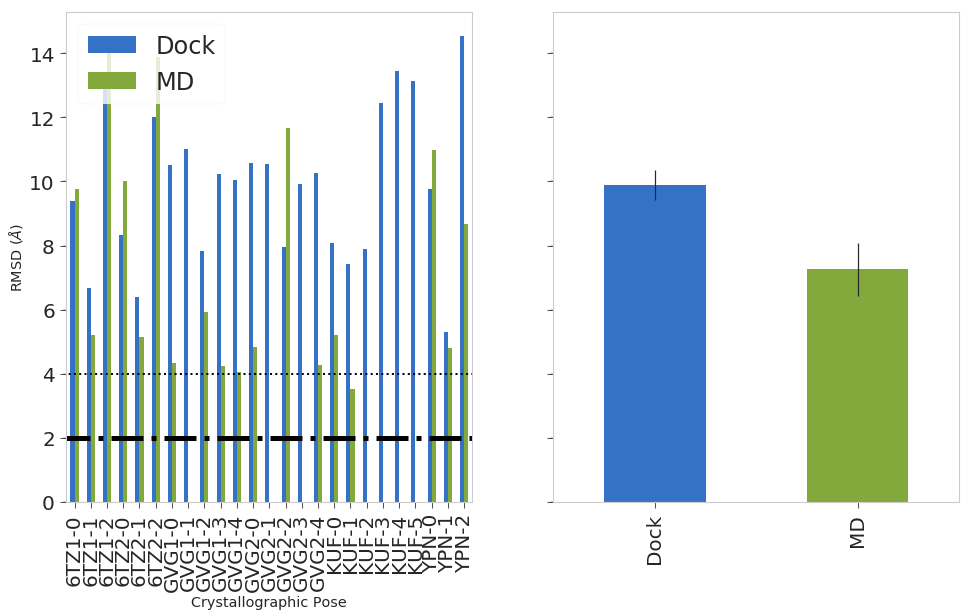
\includegraphics[width=\linewidth]{chapter5/Figures/cluster3_seh_multibm.png}
    \caption[SEH MD Multi Binding Mode Ligands]{RMSD between crystallographic ligand binding modes and predicted binding modes from docking (blue) and MD (green) for cases with multiple crystallographic binding modes. We judge success as predicting a binding mode to be less than or equal to 2 {\AA} (black dashed horizontal line).}
    \label{fig:rmsd-multibm}
\end{figure}

\begin{table}[]
\begin{tabular}{|l|l|l|l|l|}
\hline
\textbf{Ligand} & \textbf{Dock} & \textbf{DockErr} & \textbf{MD} & \textbf{MDErr} \\ \hline
\textbf{6TZ1-0} & 16.6          & \textit{0.0}     & 6.5         & \textit{0.0}   \\ \hline
\textbf{6TZ1-1} & 15.4          & \textit{0.0}     & 15.8        & \textit{0.1}   \\ \hline
\textbf{6TZ1-2} & 10.1          & \textit{0.0}     & 8.8         & \textit{0.0}   \\ \hline
\textbf{6TZ2-0} & 5.7           & \textit{0.0}     & 5.4         & \textit{0.0}   \\ \hline
\textbf{6TZ2-1} & 8.4           & \textit{0.0}     & 0.9         & \textit{0.0}   \\ \hline
\textbf{6TZ2-2} & 9.1           & \textit{0.0}     & 7.1         & \textit{0.0}   \\ \hline
\textbf{GVG1-0} & 9.4           & 0.0              & 9.8         & 0.0            \\ \hline
\textbf{GVG1-1} & 6.7           & 0.0              & 5.2         & 0.0            \\ \hline
\textbf{GVG1-2} & 13.4          & 0.0              & 14.0        & 0.0            \\ \hline
\textbf{GVG1-3} & 8.3           & 0.0              & 10.0        & 0.0            \\ \hline
\textbf{GVG1-4} & 6.4           & 0.0              & 5.1         & 0.0            \\ \hline
\textbf{GVG2-0} & 12.0          & 0.0              & 13.9        & 0.0            \\ \hline
\textbf{GVG2-1} & 10.5          & 0.0              & 4.3         & 0.0            \\ \hline
\textbf{GVG2-2} & 11.0          & 0.1              & NF          & NF             \\ \hline
\textbf{GVG2-3} & 7.8           & 0.0              & 5.9         & 0.0            \\ \hline
\textbf{GVG2-4} & 10.2          & 0.0              & 4.2         & 0.0            \\ \hline
\textbf{YPN-0}  & 10.1          & 0.0              & 4.0         & 0.0            \\ \hline
\textbf{YPN-1}  & 10.6          & 0.1              & 4.8         & 0.0            \\ \hline
\textbf{YPN-2}  & 10.6          & 0.1              & NF          & NF             \\ \hline
\textbf{KUF-0}  & 8.0           & 0.0              & 11.7        & 0.1            \\ \hline
\textbf{KUF-1}  & 9.9           & 0.0              & NF          & NF             \\ \hline
\textbf{KUF-2}  & 7.9           & 0.0              & NF          & NF             \\ \hline
\textbf{KUF-3}  & 12.5          & 0.0              & NF          & NF             \\ \hline
\textbf{KUF-4}  & 13.4          & 0.0              & NF          & NF             \\ \hline
\textbf{KUF-5}  & 13.1          & 0.0              & NF          & NF             \\ \hline
\end{tabular}
\caption[Average RMSDs and error {\AA} for molecules with multiple binding modes.]{Average RMSDs and error {\AA} for molecules with multiple binding modes. NF indicates that the binding mode was not found.}
\label{table:multibm}
\end{table}

\section{Discussion}
Our MD simulations were initiated from up to three unique docked poses, giving preference to selecting at least one docked pose for each side of the binding pocket. 
The docked poses were selected to increase the variety of starting positions for MD, ideally a docked position in the left and right sub-cavities and a docked position near the center cleft region.
Ligands with less than three poses were often a result of the docking program not placing the ligand near one of the correct region. 
Here, we hypothesized that docked poses and their scores would not adequately identify the crystallographic pose--which we confirmed at the conclusion of this study \ref{fig:topscore_correlation}.
Instead, docking was used as a means for generating starting positions for our MD simulations and hypothesized that the occupancy (i.e. amount of simulation time spent) for each binding mode would be indicative of finding the crystallographic pose.

In the 50 docked poses generated for each molecule, we found that there were indeed a handful of poses which were within 2 {\AA} of the crystallographic pose.
But, given that the docking score did not correlate with closeness to the crystallographic pose, we could not know \emph{a priori} which of the 50 docked poses represented the crystallographic binding mode.
This suggests that docking and scoring is not an effective approach in itself in general and suggests that a better method, perhaps one like MD, may be more successful at identifying dominant binding modes.

Among the bound structures considered in this study, ligands differed in how many crystallographic binding modes were resolved. 
Some had a single binding mode, others two, and some even exhibited larger numbers of binding modes.
If 1 microsecond long MD simulations were long enough to adequately sample enough binding mode transitions, we expect that the populations from MD should be roughly equivalent to the occupancies found via crystallography.
Given that, we expected fragments which exhibit a single binding mode to be easy to identify, fragments with dual binding modes to be moderately challenging, and fragments with multiple binding modes to be the most difficult.
Surprisingly, we found that 1 microsecond of MD did not result in adequate enough sampling for us to get a high success rate in identifying the crystallographic poses. 
It may be possible that an incorrect force field was selected for our system, preventing a simulation of any length from adequately sampling the binding site.
In the following sections, we present and discuss our findings for ligands which exhibited single, two, or more binding modes.

\subsection{Single binding modes: MD simulations can refine poorly docked poses}
For molecules with a single binding mode, we only had a few success cases (ONR and II6). 
Here, we present our observations from II6 to illustrate a successful scenario. 
Molecule II6 represents one case where docking does poorly, but 1 microsecond of MD results in the molecule eventually finding the crystallographic binding mode.

The other molecules in this subset (besides ONR and II6), illustrate that running 1 microsecond MD simulations after docking generally decreases the RMSD to the crystallographic binding mode, but not within the 2 {\AA} cutoff.
We believe that given more simulation time for the other molecules, we would observe similar behaviors to our observations from our II6 simulations.


\begin{figure}
    \centering
    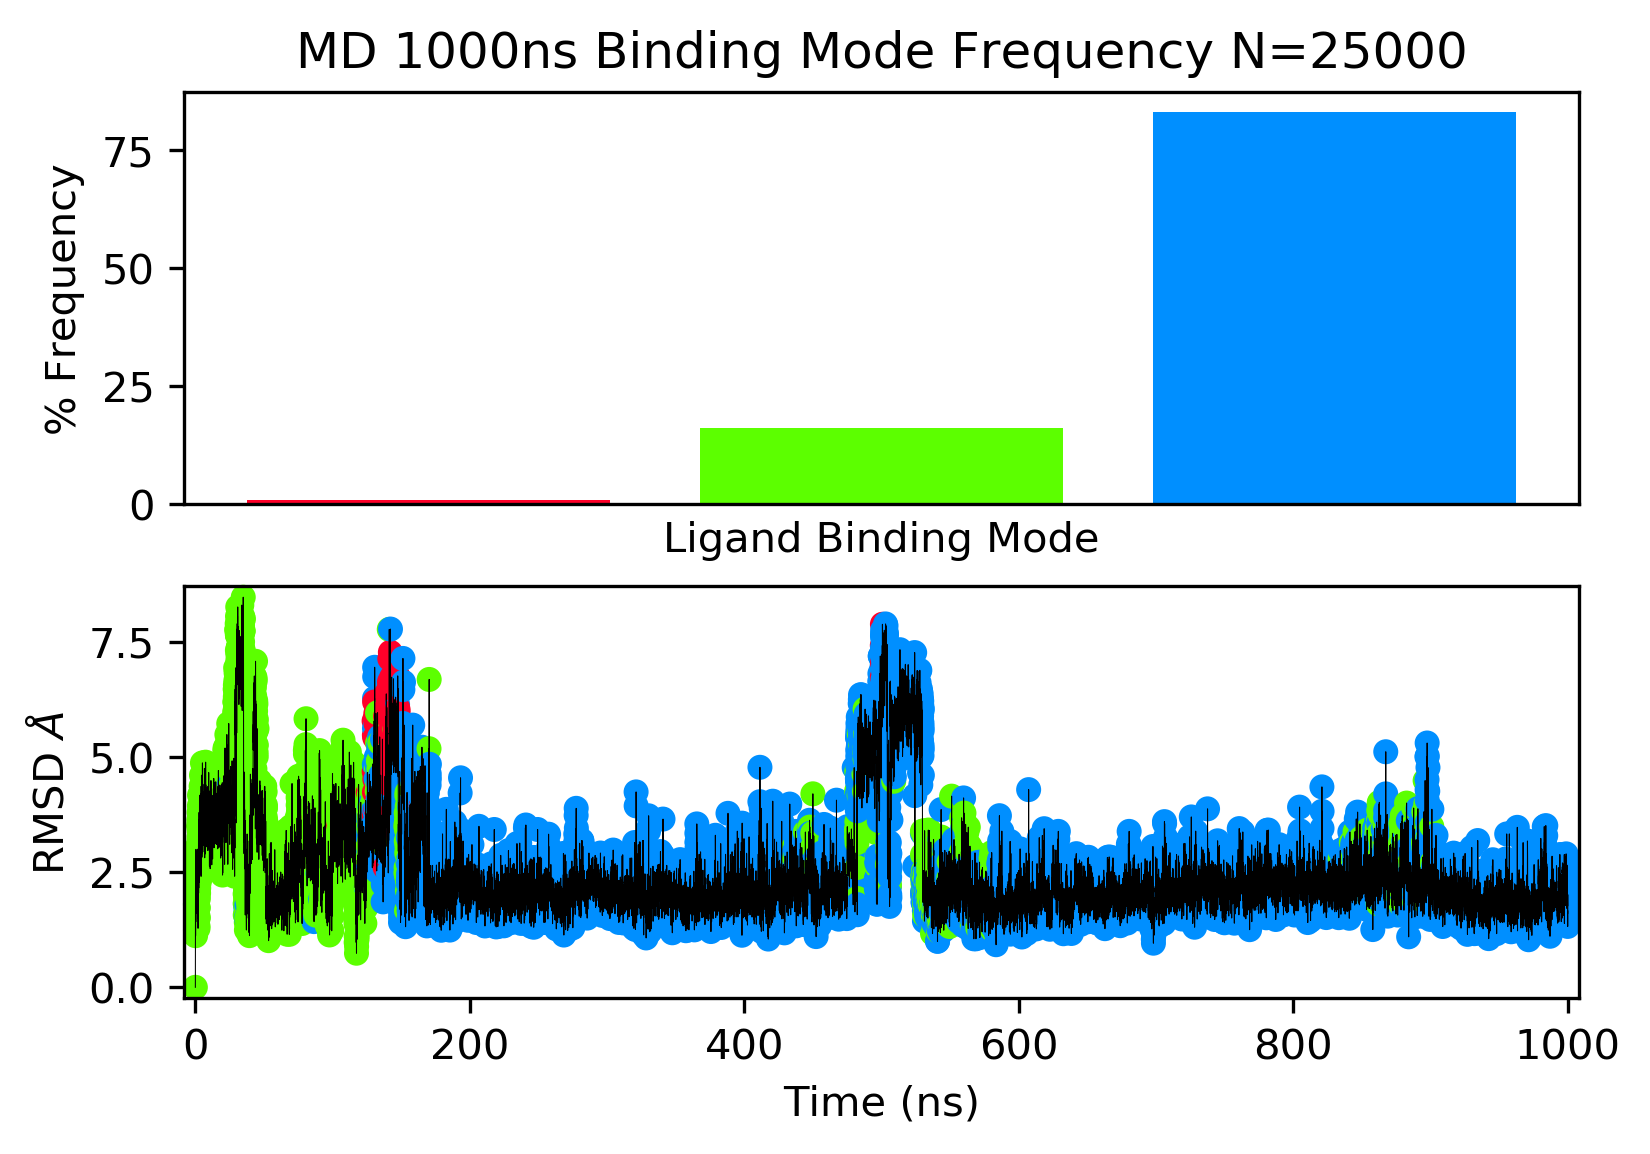
\includegraphics{chapter5/II6/II6_1-full-bmodes-freq.png}
    \caption[Ligand II6 Binding Mode Populations]{Top: Populations (\% simulation time) of 3 (red, green, blue) binding modes sampled in 1 microsecond of MD for ligand II6. Bottom: RMSD of ligand II6 relative to starting positions over time. Each time point is colored according to the binding mode the ligand is in.}
    \label{fig:II6_bmodes}
\end{figure}

Molecule II6 has one crystallographic pose (PDB:5ALL) which was not found by docking but was identified by MD.
On average, docking generated poses which were 7.9 {\AA} away from the crystallographic pose.

Our MD simulations of II6 began by selection of one docked pose situated on the right side of the SEH binding pocket.
Figure \ref{fig:II6_bmodes}, illustrates that a short amount of time (~150ns) was spent in the initial docked pose (green).
During the time spent in the initial docked pose (green), we observe high fluctuations in the ligand RMSD, indicating that docking has placed the fragment in an unfavorable pose.
After 200ns, we see a transition into a second binding mode (blue) which the fragment resides in for the remainder of the simulation, indicating favorability, representing the dominant binding mode in this simulation.
This (blue) binding mode from MD was 1.8 {\AA} away from the crystallographic pose. 

\begin{figure}
    \centering
    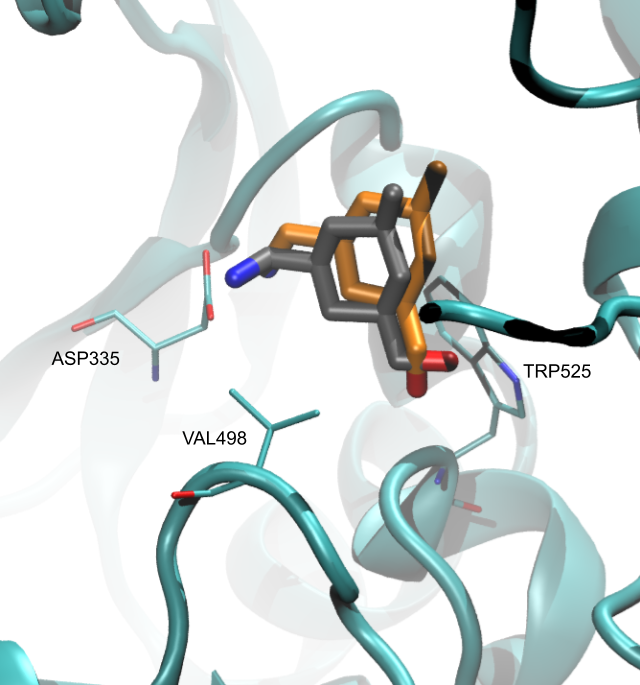
\includegraphics[width=\linewidth]{chapter5/II6/BR-II6_1-pcca2-CL.png}
    \caption[Ligand II6 with crystal structure]{The dominant binding mode for ligand II6 represented in orange and the crystallographic pose II6 in gray.}
    \label{fig:II6_pcca2}
\end{figure}

Our observations from II6 suggests that docking has a tendency to place the fragments in an unfavorable pose and that after enough simulation time, MD allows the fragment to eventually relax into a new stable configuration.
Generally, we observe the same trend with the other single binding mode fragments.
That is, docking on average does a poor job in placing the fragment in a favorable configuration but relaxation via MD allows the fragment to settle into a new stable configuration.
Once the fragment has stabilized into this new binding mode, the fragment resides there for the remainder of the simulation.
It is often this second binding mode found--following the initial pose from docking--is representative of the dominant binding mode such as in the case of II6 and ONR or somewhat close (within 4A) such as in 8NY, TGX, K2T, KJU, and 4XH (6/10 cases).
It is important to note that, in cases in which we were successful or close, the simulations started within the right sub-cavitity--a more compact region, in which ligand stabilization occurs more quickly (Fig. \ref{fig:sEH-ribbon}).
For these cases, ligand stabilization into the dominant binding mode often occurs between 200-600ns, well within the 1 microsecond timescale of our simulations.  

\begin{figure}
    \centering
    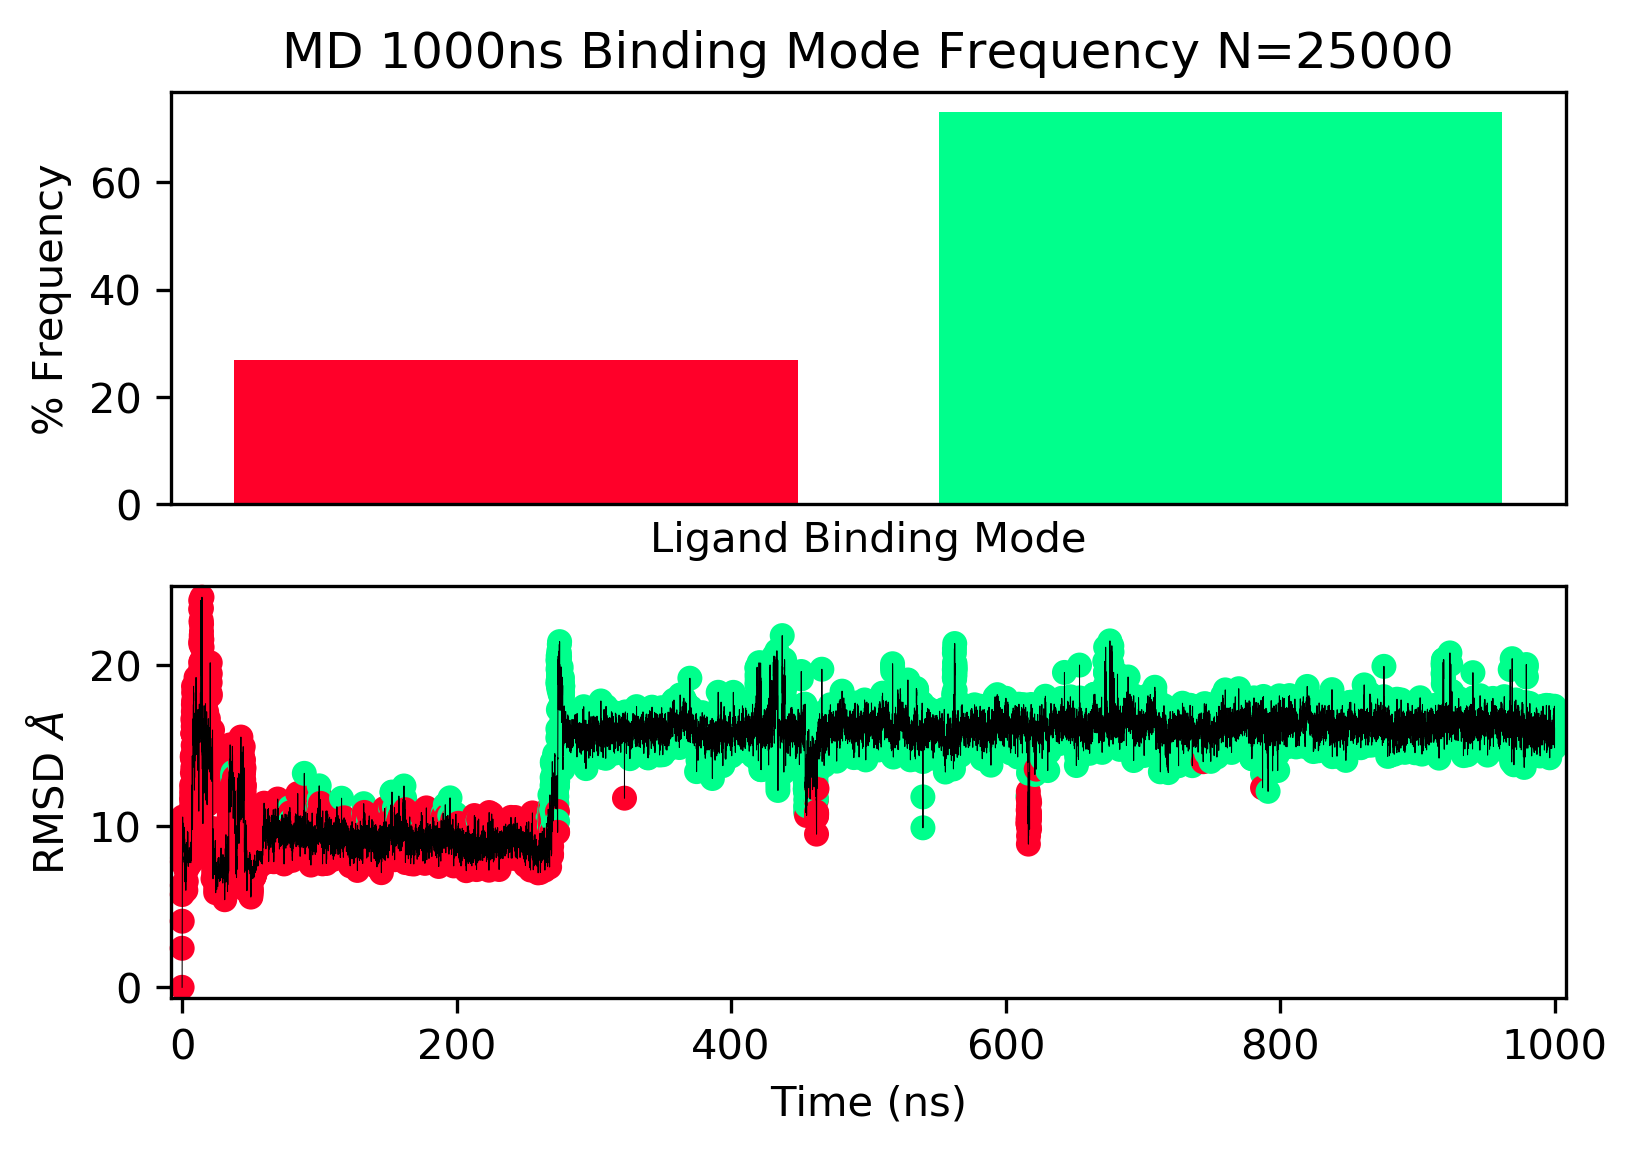
\includegraphics[width=\linewidth]{chapter5/JF6/JF6_1_c0-full-bmodes-freq.png}
    \caption[Ligand JF6 Binding Mode Populations]{Top: Populations (\% simulation time) of 2 (red and green) binding modes sampled in 1 microsecond of MD for ligand JF6. Bottom: RMSD of ligand JF6 relative to starting positions over time. Each time point is colored according to the binding mode the ligand is in.}
    \label{fig:JF6_bmodes}
\end{figure}

Crystallographic poses for JF6, 6N4, and 6N6 were found to be in the left side of the binding site, where the pocket is much larger and wider.
The larger sub-cavity allows for there to be many more possible metastabile binding modes that the ligand here explores only slowly because of barriers separating them.
Given this, it is unsurprising that we performed poorly in trying to identify the crystallographic pose via MD.
Here, a larger pocket means we must simulate long enough for the fragment to wander away from the initial docked pose and explore enough different metastable binding modes that it can find the dominant binding mode and remain there for a long period of time.
From figure \ref{fig:JF6_bmodes}, we see that JF6 begins in the initial (red) docked pose and then deviates up to 15 {\AA} away into another binding mode (green).
This (green) binding mode was 5.4 {\AA} away from the crystallographic pose, which is likely a result from not allowing enough simulation time for the fragment to find a more favorable binding mode.
On average, the poses generated from docking were 14.6 {\AA} away from the crystallographic pose.
These findings suggest that for larger pockets, one may need to simulate longer than 1 microsecond in order to get enough simulation time to recover from poor initial placements from docking.

\subsection{Dual and Multiple binding modes: Microsecond MD simulations do not capture enough binding mode transitions}
Here, we present our observations on simulations of 6NX, the sole success case in the subset of ligands which have more than one binding mode.
Generally, across this subset of molecules with multiple binding modes, our observations suggest that 1 microsecond of MD simulations do not capture enough binding mode transitions for us to successfully find the correct dominant binding mode.
In our single successful case of identifying 1 binding mode for 6NX, we do not observe any transitions during the course of the simulation, which furthers our claim that 1 microsecond of MD simulations is not sufficient enough of a timescale to get the correct populations for finding the crystallographic binding mode.

Molecule 6NX has two crystallographic poses (PDB:5AKZ), referred to as 6NX-0 and 6NX-1.
The two crystallographic binding poses for 6NX are located by the cleft region of the SEH binding pocket, on the left side of the protein. 
On average, docking generated poses which were 8.4 {\AA} from 6NX-0 and 9.1 {\AA} from 6NX-1. 

\begin{figure}
    \centering
    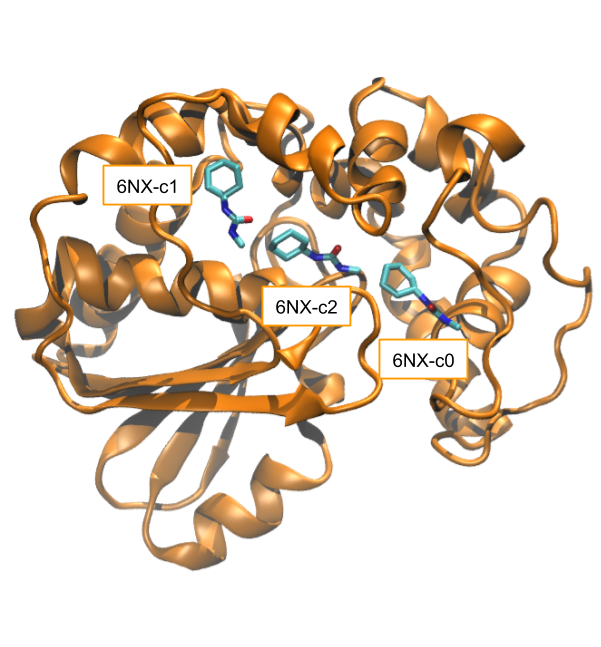
\includegraphics[width=\linewidth]{chapter5/6NX/6NX-docked-label.png}
    \caption[Ligand 6NX Docked Poses]{Ligand 6NX in the 3 chosen docked poses 6NX-c0 (right), 6NX-c1 (left), and 6NX-c2 (left) used to start our MD simulations.}
    \label{fig:6NX-docked}
\end{figure}

Our MD simulations of 6NX began by selection of three uniquely docked poses named 6NX-c0, 6NX-c1, and 6NX-c2 situated on the right, left, and left side of the of the SEH binding pocket, respectively \ref{fig:6NX-docked}. 
Populations from MD simulations that are on the same side of the binding site were combined, therefore 6NX-c1 and 6NX-c2 simulations were combined and 6NX-c0 was analyzed separately.
Populations for 6NX-c0 are not included in this analysis because the crystallographic binding modes are not located in the right side of the binding pocket.
The populations of 6NX-c1 and 6NX-c2 are combined to yield red, green, and blue binding modes with populations of 16\% , 34\% , and 50\% , respectively (Fig. \ref{fig:6NX_c2_bmodes} and Fig. \ref{fig:6NX_c1_bmodes}). 

\begin{figure}
    \centering
    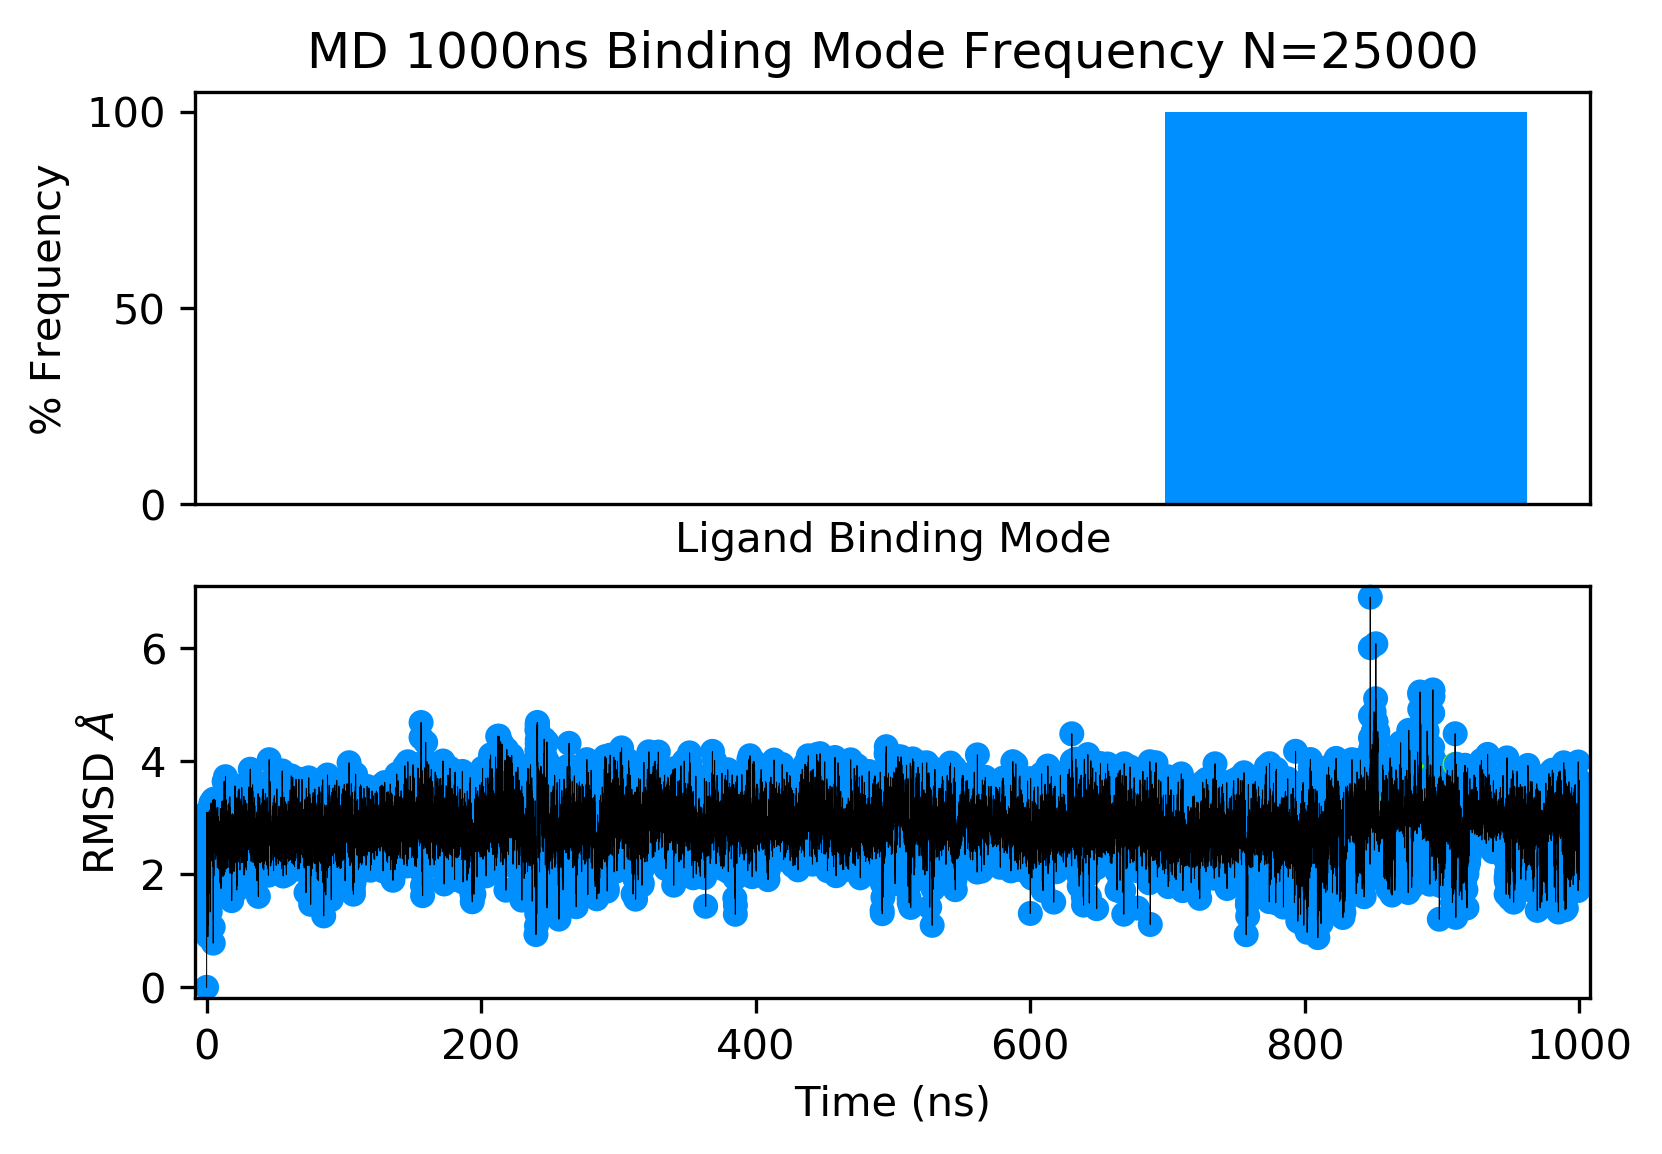
\includegraphics[width=\linewidth]{chapter5/6NX/6NX_1_c2-full-bmodes-freq.png}
    \caption[Ligand 6NX pose 2 Binding Mode Populations]{Top: Populations (\% simulation time) of 1 (blue) binding modes sampled in 1 microsecond of MD for ligand 6NX (pose 2). Bottom: RMSD of ligand 6NX relative to starting positions over time. Each time point is colored according to the binding mode the ligand is in.}
    \label{fig:6NX_c2_bmodes}
\end{figure}
Figure \ref{fig:6NX_c2_bmodes} illustrates that 6NX-c2 in the cleft region of the SEH binding site (left side) spent the entirety of the simulation in the initial docked pose (blue) and does not transition to any additional binding mode.
This is indicative that binding mode transitions for this particular ligand is either very slow or that additional simulation time is required for observing a transition out of this initial binding mode.
By chance, the docked pose 6NX-c2 we selected as a starting point for our MD simulations, was already close to the crystallographic pose by 0.9 {\AA} which likely partialy explains the lack of binding mode transitions in this simulation.


\begin{figure}
    \centering
    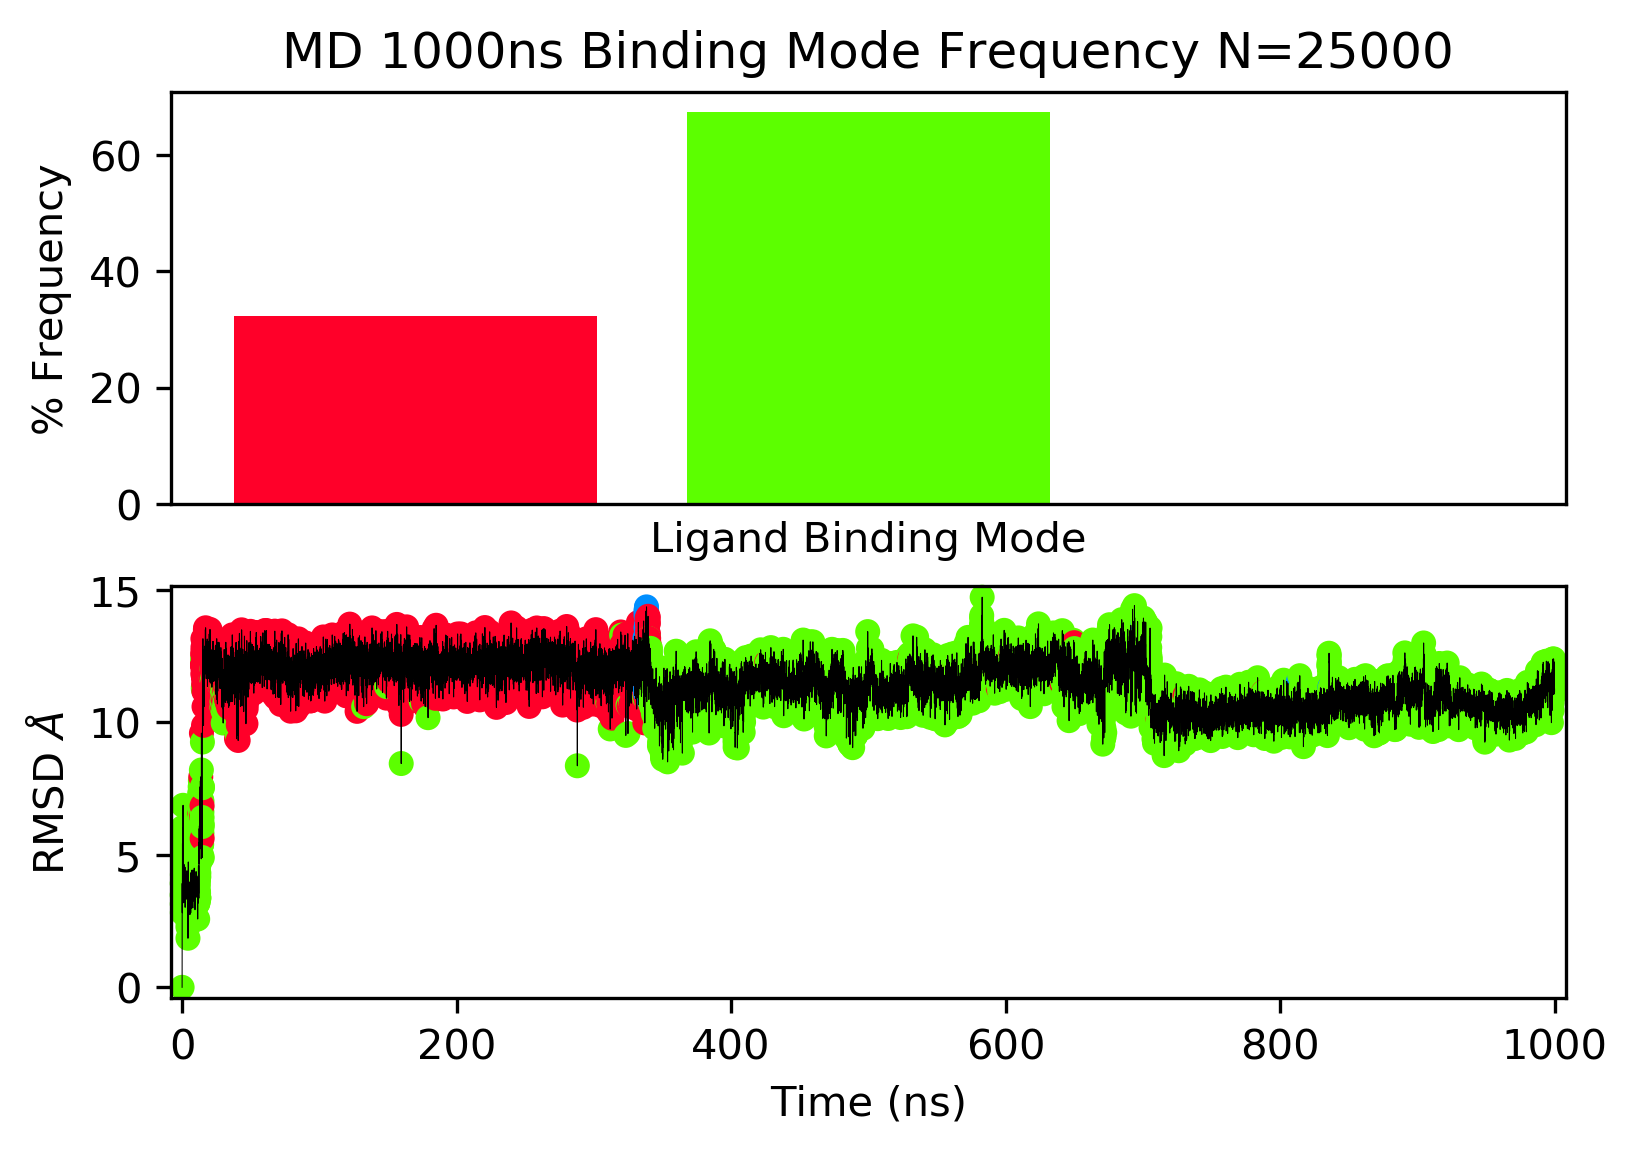
\includegraphics[width=\linewidth]{chapter5/6NX/6NX_1_c1-full-bmodes-freq.png}
    \caption[Ligand 6NX pose 1 Binding Mode Populations]{Top: Populations (\% simulation time) of 2 (red/green) binding modes sampled in 1 microsecond of MD for ligand 6NX (pose 1). Bottom: RMSD of ligand 6NX relative to starting positions over time. Each time point is colored according to the binding mode the ligand is in.}
    \label{fig:6NX_c1_bmodes}
\end{figure}

Figure \ref{fig:6NX_c1_bmodes} shows that 6NX-c1 on the left of the binding pocket begins in the initial docked pose (red) and has high fluctuations in the ligand RMSD during the first ~30ns of the simulation.
The red binding mode remains for approximately ~325ns, then transitions to another binding mode (green), where it remains till the end of the simulation (~675ns).
This secondary binding mode (green) was 7.1 {\AA} away from the secondary crystallographic binding mode.
In this case, we see that from the initial docked pose the ligand drifts ~12{\AA} away over the course of the 1 microsecond MD simulation.
Here, docking had placed the ligand so far away from the crystallographic pose that the simulation was not long enough for the ligand to find the second crystallographic pose (6NX-1).

In the case of 6NX, even with two simulated poses on the same side of the binding site exploring three total different binding modes, 1 microsecond of MD simulations was not sufficient to identify both crystallographic poses.
In one simulation (6NX-c1), we happened to select a docked pose that was very close to one of the crystallographic poses but saw no binding mode transitions during the MD simulation to uncover the secondary binding mode.
In our other simulation (6NX-c2), docking had poorly placed the ligand so far away that we our simulations did not sample either of the crystallographic poses.
In this case, MD captured only one binding mode transition from one simulated pose (6NX-c2), but neither the binding modes sampled were close to the crystallographic poses due to poor initial placement from docking. 

Our observations from 6NX indicate that 1 microsecond of MD does not sufficiently capture enough binding mode transitions, nor does it appear to be a long enough timescale to correct the poor placements from docking.
We observe the same trend with the other fragments, where there is a lack of binding mode transitions, only seeing at most 3 transitions per simulation.
In all (dual and multiple) binding mode cases but one, neither docking or 1 microsecond of MD proved sufficient in identifying the crystallographic binding modes.
Had the microsecond timescale been sufficient to reliably sample at least two binding modes, we would have at least observed a transition in the 6NX-c1 simulation, allowing us to potentially find the secondary binding mode.
Our findings suggest that MD simulations at the microsecond timescale may be able to find at least one crystallographic pose, but identifying secondary or even more binding modes is not likely without much longer simulations. 

\section{Conclusion}
In this study, we used docking and MD on a set of fragment-like molecules binding to soluble epoxide hydrolase to evaluate each method's effectiveness in predicting the crystallographic poses and whether sufficient sampling of relevant fragment binding modes can occur at a 1 microsecond timescale.
Although docking typically produces a few poses close to the crystallographic binding mode, docking on average performs poorly in predicting the crystallographic binding mode.
Our findings show that in the case of fragments with a single binding mode, a relatively small amount of MD  (~250ns) can refine the poses generated from docking and get close to identifying the crystallographic pose. 
In cases where there are multiple binding modes, we anticipated observing multiple binding mode transitions based on the fragment sized ligands and the relatively weak binding such molecules typically exhibit. However we generally do not see more than 3 transitions in our simulations.
MD may find one crystallographic binding mode, however the lack of binding mode transitions restricts MD from revealing multiple crystallographic binding modes despite simulating for a relatively long timescale of 1 microsecond.
Here, the binding site of SEH was relatively large and we divided the entirety of the binding site into two sub-cavities, expecting to observe transitions between them.
However, transitions between the divided sub-cavities of SEH were rarely observed in our simulations of the molecules on a microsecond timescale.
Without more binding mode transitions, we cannot rely on the populations from MD because we do not observe enough binding mode transitions at the microsecond timescale. 

This highlights the necessity of using enhanced sampling techniques in the future, which could help address the fact that microsecond MD simulations did capture multiple binding mode transitions or transition between sub-cavities.
Improved sampling would allow better predictions of ligand binding modes and collection of more accurate populations, which we could use to identify the ligand binding modes that would be found in crystallography.
In this study, we effectively selected docked poses at random to initiate our MD simulations, but for the most part, these docked poses were too far away from the crystallographic pose in that a microsecond MD simulation was not sufficient enough of a timescale to allow for finding the crystallographic pose.

Instead, future studies could investigate using an automated protocol for selecting a more diverse set of docked poses to have a larger variety of poses as starting structures for our MD simulations.
A wider selection of docked poses could improve the chances that refinement by short MD simulations of approximately 250ns would result in finding the crystallographic binding modes. 
Though, this process could generate multiple poses not related to the experimental binding modes.
This improved approach for selecting initial docked poses in combination with enhanced sampling techniques, could result in starting closer to equilibrium during our simulations, where we would observe sufficient enough transitions between the relevant ligand binding modes.
Through proper sampling, we could rely on the populations in our simulations to determine the likely binding modes as found by crystallography.
An alternate approach which can supplement the analysis of populations is to analyze protein-ligand contacts.

In this study, we show that even when simulating small fragment-like molecules in a large spacious binding pocket, sampling reasonable ligand binding mode transitions is challenging, even with relatively long MD simulations.
This illus rates that convergence, solely with MD simulations, is very slow and highlights the necessity of using an enhanced sampling technique to adequately sample and determine ligand binding modes.
We plan to explore these issues in future work.

% \section{Contributors}
% Christopher Bayly -- OpenEye Scientific, provided MD Floes
% Gaetano Calabro -- OpenEye Scientific, provided MD Floes
% Greg Warren -- OpenEye Scientific,  curated crystal structures

\section{Acknowledgements}
DLM appreciates financial support from the National Institutes of Health (1R01GM108889-01 and 1R01GM124270-01A1). Financial support for N.M.L. was provided by the National Science Foundation Graduate Research Fellowship (DGE-1321846)

